%% Tato práce je psána na vzoru do MFF UK, který jsem hodně osekal
\documentclass[12pt,a4paper]{report}
%% Verze pro jednostranný tisk:
% Okraje: levý 40mm, pravý 25mm, horní a dolní 25mm
% (ale pozor, LaTeX si sám přidává 1in)

\setlength\textwidth{145mm}
\setlength\textheight{247mm}
\setlength\oddsidemargin{15mm}
\setlength\evensidemargin{15mm}
\setlength\topmargin{0mm}
\setlength\headsep{0mm}
\setlength\headheight{0mm}
% \openright zařídí, aby následující text začínal na pravé straně knihy
\let\openright=\clearpage

%% Pokud tiskneme oboustranně:
% \documentclass[12pt,a4paper,twoside,openright]{report}
% \setlength\textwidth{145mm}
% \setlength\textheight{247mm}
% \setlength\oddsidemargin{14.2mm}
% \setlength\evensidemargin{0mm}
% \setlength\topmargin{0mm}
% \setlength\headsep{0mm}
% \setlength\headheight{0mm}
% \let\openright=\cleardoublepage

%% Vytváříme PDF/A-2u
\usepackage[a-2u]{pdfx}

%% Přepneme na českou sazbu a fonty Latin Modern
\usepackage[czech]{babel}
\usepackage{lmodern}
\usepackage[T1]{fontenc}
\usepackage{textcomp}

%% Použité kódování znaků: obvykle latin2, cp1250 nebo utf8:
\usepackage[utf8]{inputenc}
\usepackage{csquotes}

%%% Další užitečné balíčky (jsou součástí běžných distribucí LaTeXu)
\usepackage{amsmath}        % rozšíření pro sazbu matematiky
\usepackage{amsfonts}       % matematické fonty
\usepackage{amsthm}         % sazba vět, definic apod.
\usepackage{amssymb}
\usepackage{bbding}         % balíček s nejrůznějšími symboly
% (čtverečky, hvězdičky, tužtičky, nůžtičky, ...)
\usepackage{bm}             % tučné symboly (příkaz \bm)
\usepackage{graphicx}       % vkládání obrázků
\graphicspath{ {img} }
\usepackage{fancyvrb}       % vylepšené prostředí pro strojové písmo
\usepackage{indentfirst}    % zavede odsazení 1. odstavce kapitoly     

\usepackage[backend=biber,style=numeric,sorting=ynt]{biblatex}
\addbibresource{zdroje.bib}

\usepackage{icomma}         % inteligetní čárka v matematickém módu
\usepackage{dcolumn}        % lepší zarovnání sloupců v tabulkách
\usepackage{booktabs}       % lepší vodorovné linky v tabulkách
\usepackage{paralist}       % lepší enumerate a itemize
\usepackage{xcolor}         % barevná sazba

\usepackage{setspace}		% řádkování

%% Fix pro cmidrule and cline kvůli češtině
\usepackage{regexpatch}
\makeatletter
% Change the `-` delimiter to an active character
\xpatchparametertext\@@@cmidrule{-}{\cA-}{}{}
\xpatchparametertext\@cline{-}{\cA-}{}{}
\makeatother


%%% Údaje o práci
\title{
        {\Huge Tvorba sbírky planimetrických a stereometrických úloh}\\
    {\large Ročníková práce}\\
    {
\includegraphics[width=0.4\textwidth]{mensa_logo_s_nazvem}}\\
    {\large Mensa gymnázium, o.p.s.}
}
\author{
        {\Large Jan Strmiska}
}
\date{
    2021 - 2023
}

%% Balíček hyperref, kterým jdou vyrábět klikací odkazy v PDF,
%% ale hlavně ho používáme k uložení metadat do PDF (včetně obsahu).
%% Většinu nastavítek přednastaví balíček pdfx.
\hypersetup{unicode}
\hypersetup{breaklinks=true}

%% Znak obdelník
\newcommand{\rectangle}{\ooalign{$\sqsubset\mkern2mu$\cr$\mkern9mu\sqsupset$\cr}}

%% Nadpis kapitoly fix
\makeatletter
\def\@makechapterhead#1{
        {\parindent \z@ \raggedright \normalfont
    \Huge\bfseries \thechapter. #1
    \par\nobreak
    \vskip 20\p@
    }}
\def\@makeschapterhead#1{
        {\parindent \z@ \raggedright \normalfont
    \Huge\bfseries #1
    \par\nobreak
    \vskip 20\p@
    }}
\makeatother

\begin{document}
%% Titulní strana a různé povinné informační strany
    %%% Titulní strana práce

\pagestyle{empty}
\hypersetup{pageanchor=false}

\maketitle

\openright
\hypersetup{pageanchor=true}
\pagestyle{plain}
\pagenumbering{roman}

2. strana
\newpage
3. strana
\newpage


\vglue 0pt plus 1fill


\noindent
Prohlašuji, že jsem svou práci vypracoval samostatně a použil jsem pouze podklady (literaturu, SW atd.) uvedené v přiloženém seznamu.

\medskip\noindent
Nemám závažný důvod proti zpřístupňování této práce v souladu se zákonem č. 121/2000 Sb., o právu autorském, o právech souvisejících s právem autorským a o změně některých zákonů (autorský zákon) v platném znění.

\vspace{10mm}

\hbox{\hbox to 0.5\hsize{%
    V \hbox to 6em{\dotfill} dne \hbox to 6em{\dotfill}
    \hss}\hbox to 0.5\hsize{\dotfill\quad}}
\smallskip
\hbox{\hbox to 0.5\hsize{}\hbox to 0.5\hsize{\hfil Podpis autora\hfil}}

\vspace{20mm}
\newpage

\openright

\noindent %Poděkování
Chtěl bych poděkovat svému vedoucímu ročníkové práce Mgr. Matúši Kepičovi za odborné vedení, za pomoc a rady při zpracování této práce.


\newpage

\openright
\pagestyle{plain}
\pagenumbering{arabic}
\setcounter{page}{1}


%%% Jednotlivé kapitoly práce jsou pro přehlednost uloženy v samostatných souborech
    \onehalfspacing
    \chapter*{Úvod}
\addcontentsline{toc}{chapter}{Úvod}

Tato ročníková práce se zaměřuje na tvorbu sbírky planimetrických a stereometrických příkladů, která má pomoci studentům připravujícím se na střední školy a gymnázia. Výběr téma je motivován mým zájmem o tuto oblast matematiky a mými zkušenostmi s tím, jak někteří studenti mohou s těmito druhy úloh bojovat.

Práce se dělí na teoretickou část, vysvětlující jednotné přijímací zkoušky a~teoretický základ, na praktickou část, ve které je popsán postup tvorby sbírky a~na samotnou sbírku úloh.

Cílem sbírky je poskytnout přehledný materiál, který studentům umožní osvojit si potřebné dovednosti k řešení planimetrických a stereometrických úloh.

Sbírka bude strukturována dle témat jednotlivých úloh a bude přehledně čitelná a vizuálně přitažlivá.

Mým hlavním zdrojem jsou jednotné přijímací zkoušky z matematiky z minulých let. Také jsem se inspiroval různými sbírkami.

V rámci této práce je předpokládáno, že studenti již mají osvojenou znalost planimetrických a stereometrických konceptů, kterou získali v rámci školní výuky. Sbírka bude tedy obsahovat především různorodé příklady, které studentům umožní procvičit a zlepšit si své schopnosti v dané oblasti.


    \chapter{Teoretická část}


\section[Jednotné přijímací zkoušky pro střední školy a gymnázia]{Jednotné přijímací zkoušky\\pro střední školy a gymnázia}

Přijímací zkoušky tvoří příspěvková organizace CERMAT neboli Centrum pro zjišťování výsledků vzdělávání, která byla zřízena Ministerstvem školství, mládeže a tělovýchovy ČR v roce 2006.~\cite{zakon_CERMAT} Tato organizace také zařizuje státní maturitní zkoušky a závěrečné zkoušky.~\cite{CERMAT_p_m}



Jde o národně jednotné přijímací zkoušky, které jsou povinnou součástí prvního kola přijímacího řízení do všech maturitních oborů s výjimkou oborů s talentovou zkouškou a oborů zkráceného studia.

„Jednotná přijímací zkouška se skládá ze dvou písemných testů - z českého jazyka a literatury a z matematiky.
Varianty testů jsou různé pro čtyřleté obory vzdělání (včetně oborů nástavbového studia), pro šestiletá gymnázia a pro osmiletá gymnázia.
Maximální možný počet dosažených bodů v testech z matematiky i českého jazyka a literatury je 50 bodů.”~\cite{CERMAT_co_to_je}

V České republice byly jednotné přijímací zkoušky testovány v letech 2015 a~2016, povinně zavedeny byly v roce 2017.~\cite{CERMAT_rocni_zprava}

Přijímací zkoušky z předchozích roků jsou dostupné na webových stránkách Centra pro zjišťování výsledků vzdělávání.~\cite{CERMAT_pdfka}


\section{Vysvětlení teoretických základů}

\subsection{Obvod}
Obvod je součet délek čar, které vymezují nějaký útvar.~\cite{umim_mat}

\begin{figure}[h]
    \centering
    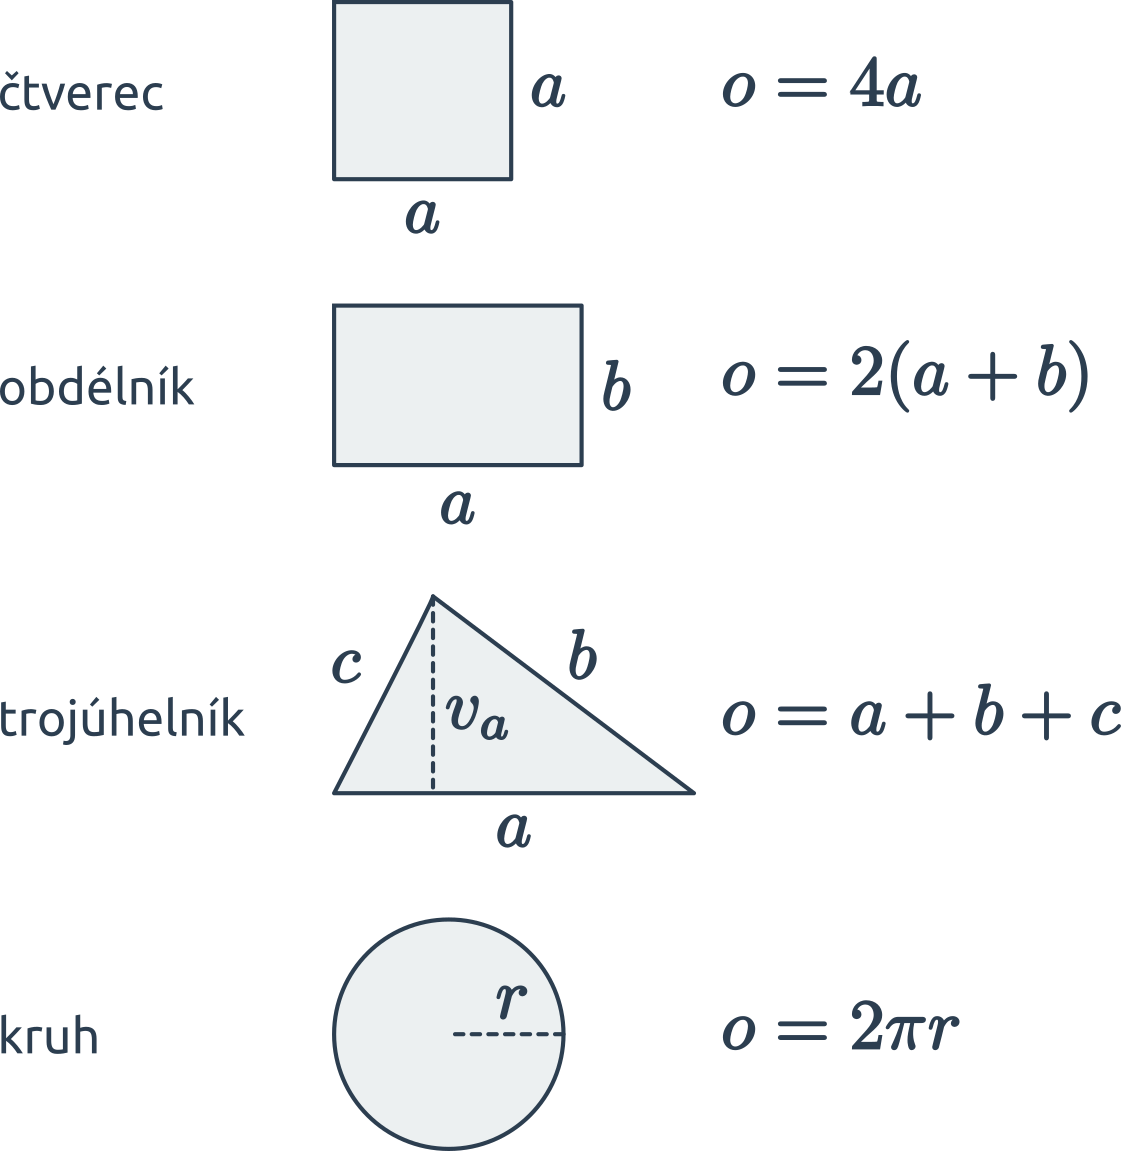
\includegraphics[width=0.6\textwidth]{teor/obvod}
    \caption{Vzorce pro výpočet obvodu~\cite{umim_mat}}
\end{figure}

Ve čtvercové síti lze obvod spočítat sečtením všech čar, které útvar tvoří. Pokud čáry nevedou rovnoběžně se sítí, můžeme je i přesto odečítat.

\subsubsection{Příklad}
\begin{minipage}[t]{\linewidth}
    Pokud chceme znát rozdíl obvodů těchto dvou tvarů, nemusíme znát oba dva obvody. U obou tvarů neznáme délku čáry, která není rovnoběžná se sítí. Víme ale, že jsou stejně dlouhé. Můžeme je tedy odečíst a pak počítat s rozdíly zbytku, které dokážeme jednoduše určit.

    Pokud je délka strany čtverce, ze kterého je čtvercové pole 1 cm, rozdíl obvodů jsou 2 cm.
    \begin{center}
        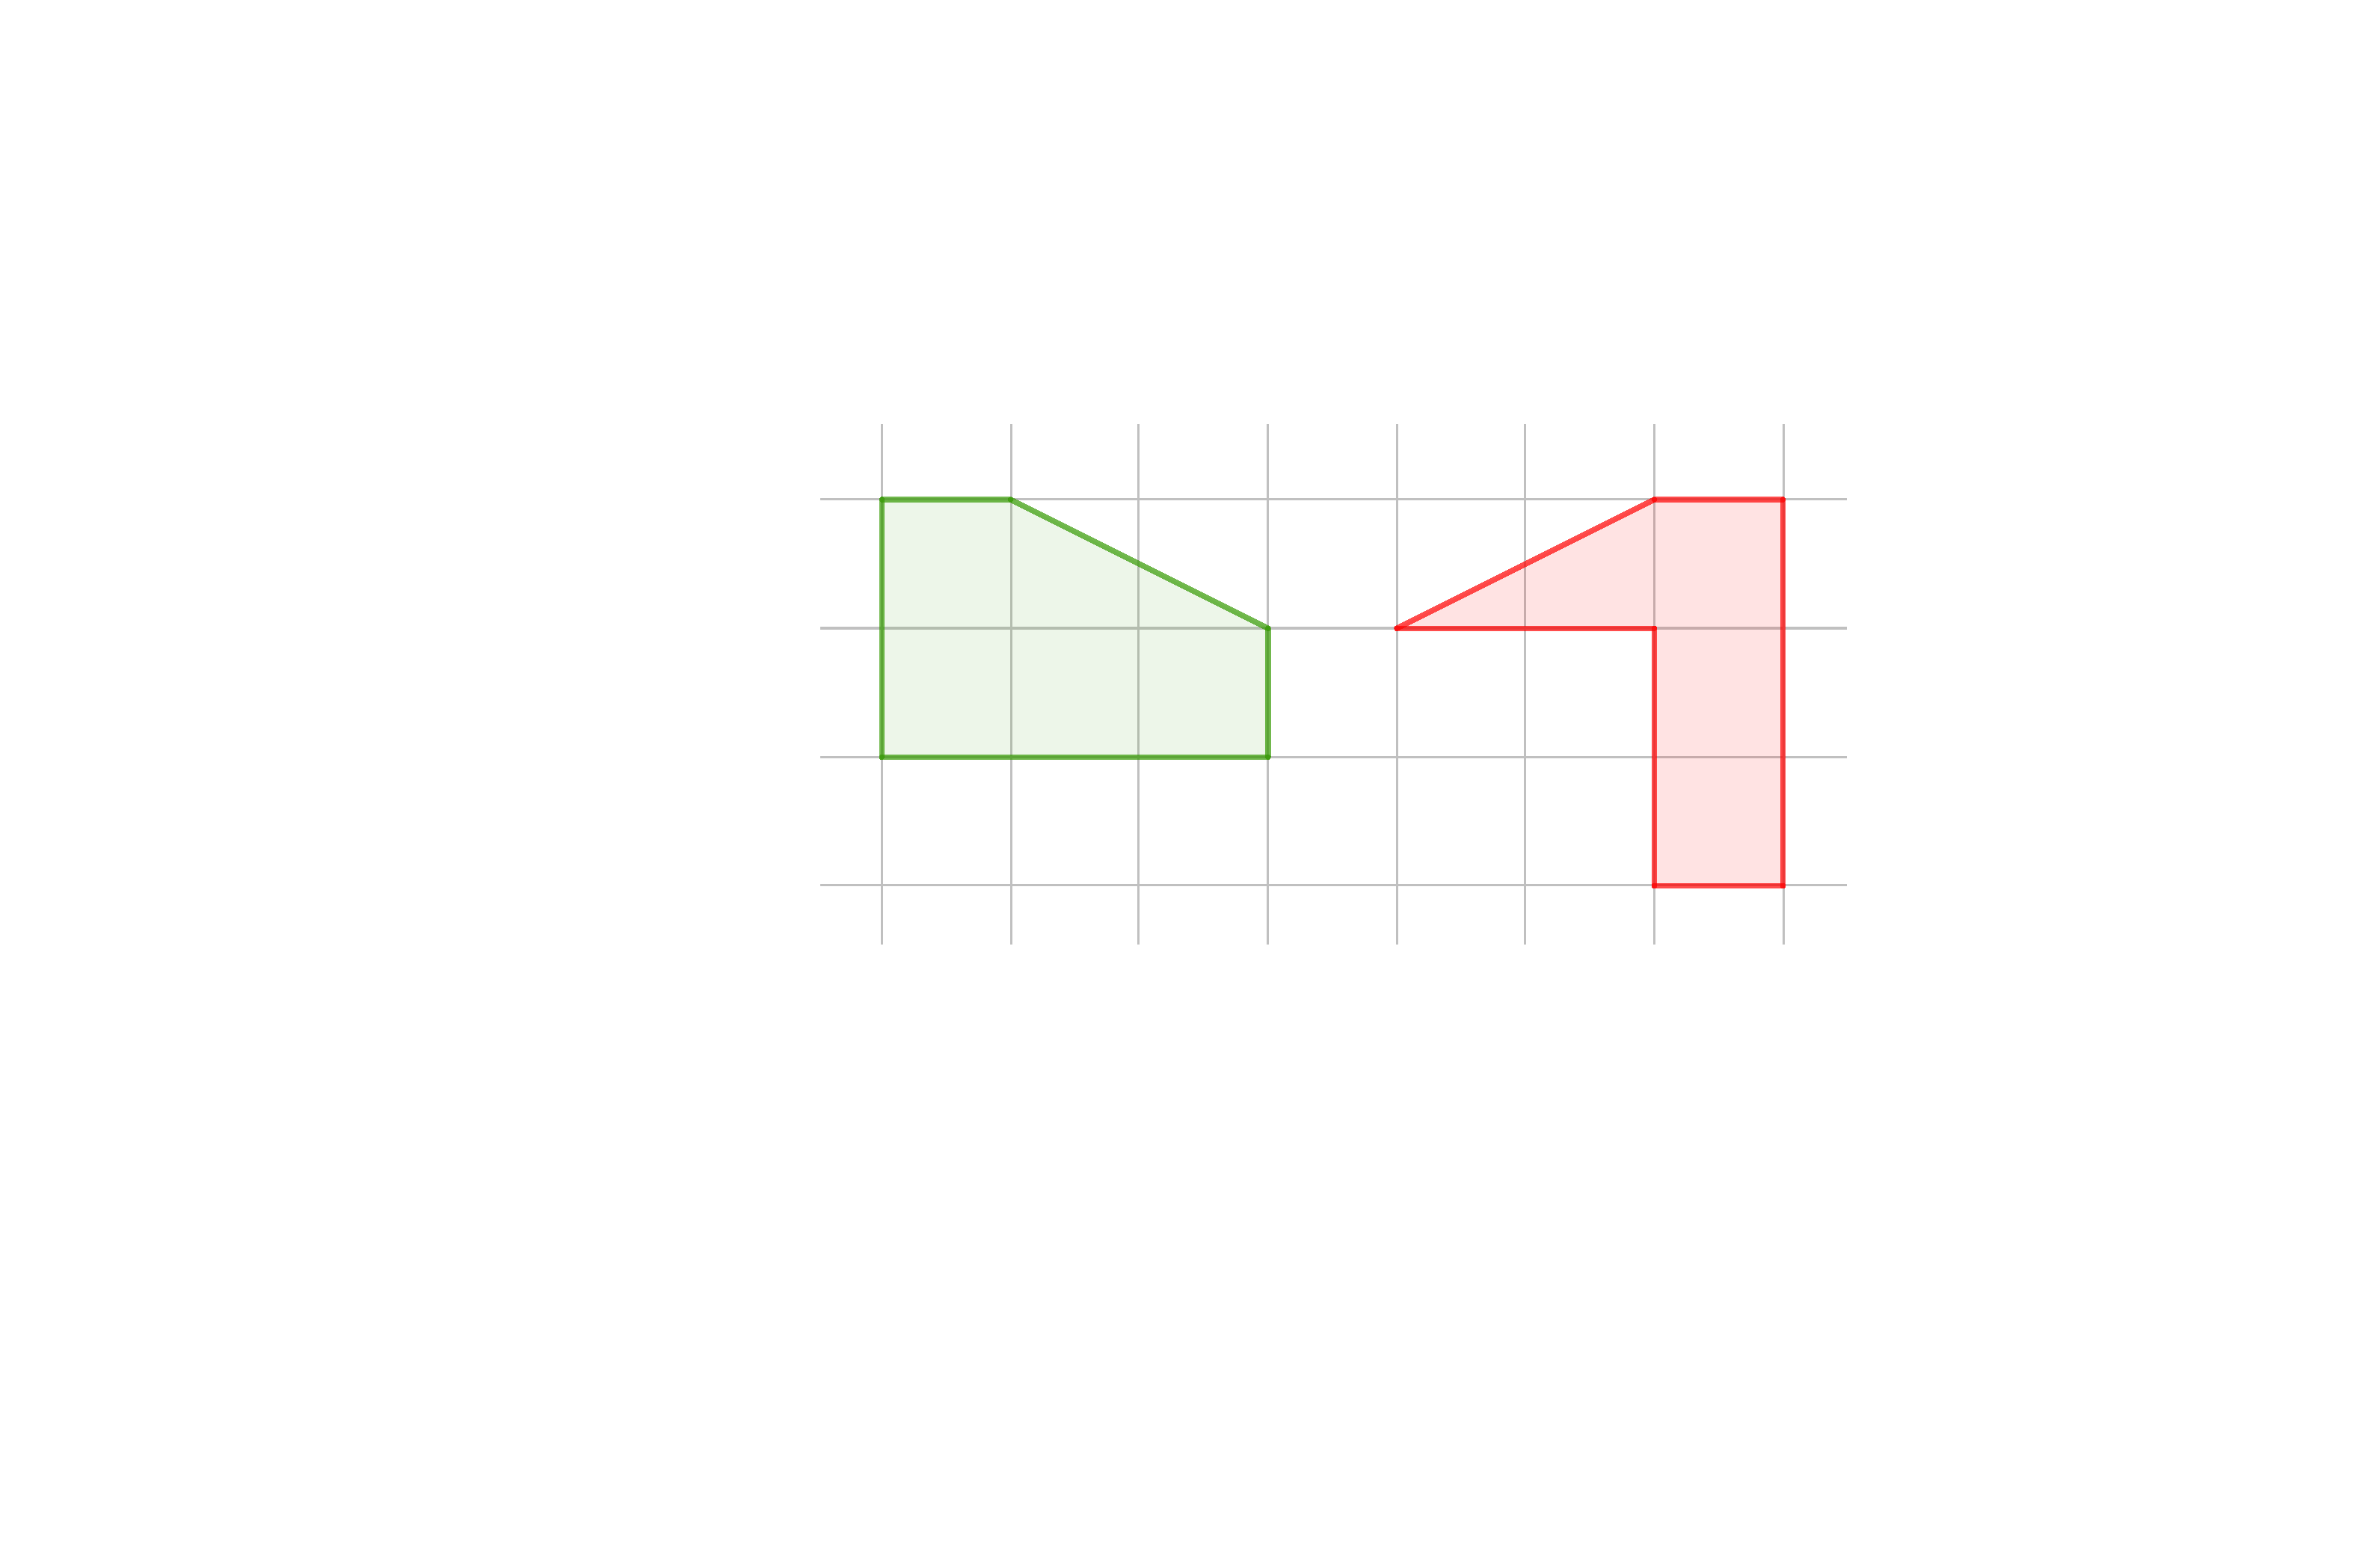
\includegraphics[width=0.6\textwidth]{teor/priklad-obvod}
    \end{center}
\end{minipage}

\subsection{Obsah}
Obsah vyjadřuje, kolik „místa v rovině“ útvar zaujímá. Měří se v jednotkách obsahu.~\cite{umim_mat}

Příkladem jednotek obsahu jsou centimetry čtvereční ($\text{cm}^{2}$) nebo metry čtvereční ($\text{m}^{2}$).



K výpočtu obsahu je nejdůležitější pamatovat si vzorce. Pokud je útvar složitý, budeme jich muset použít několik.

\begin{figure}[h]
	\centering
	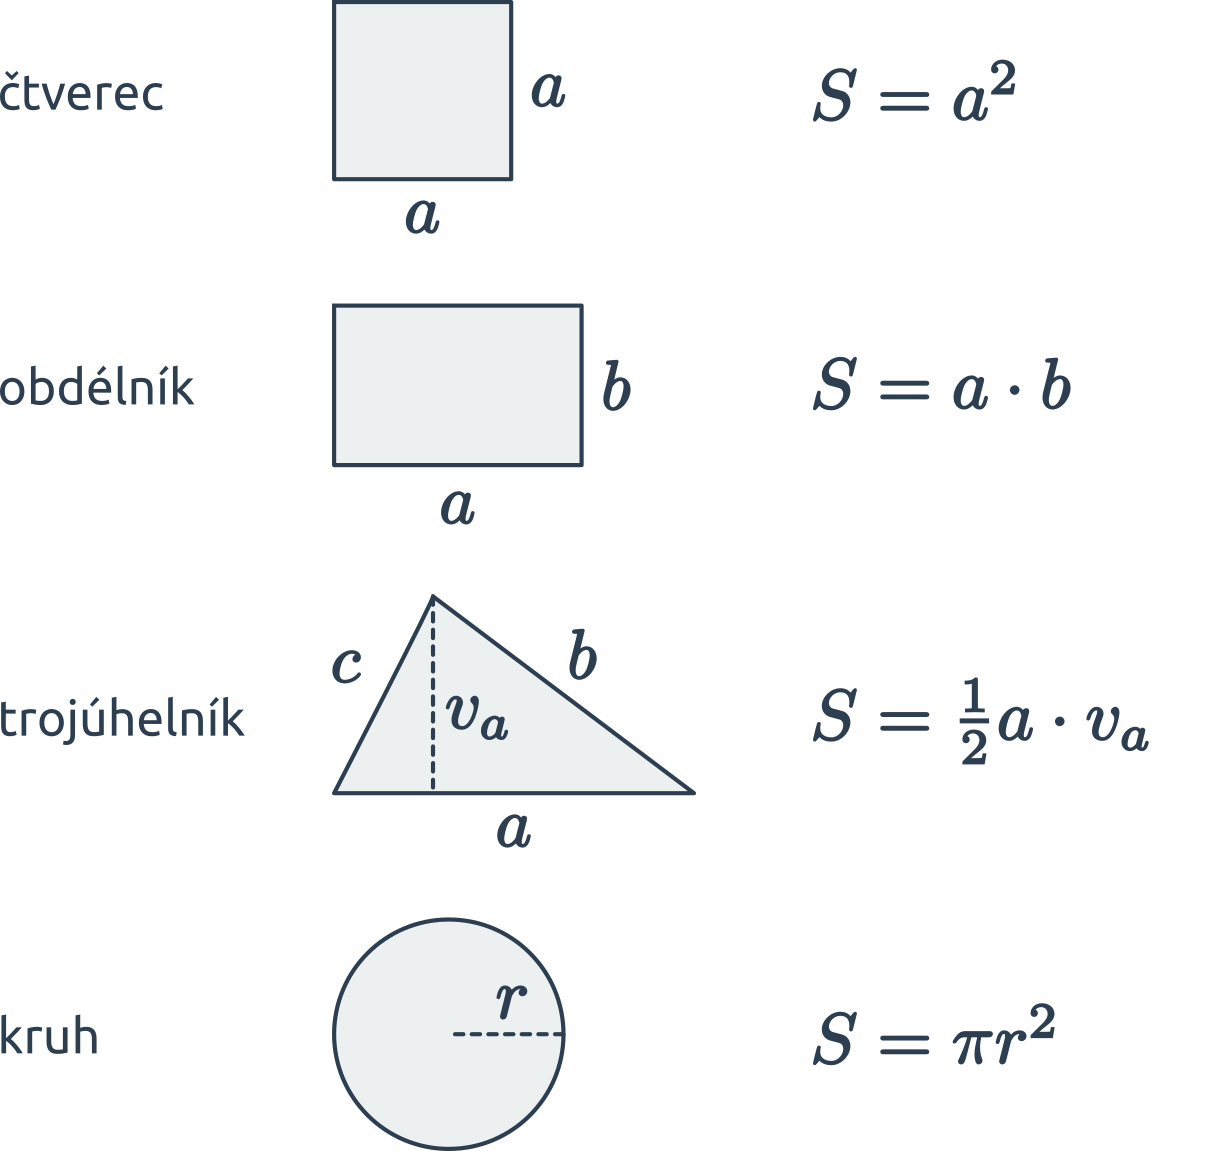
\includegraphics[width=0.6\textwidth]{teor/obsah}
	\caption{Vzorce pro výpočet obsahu~\cite{umim_mat}}
\end{figure}

\subsubsection{Příklad}
\begin{minipage}[t]{\linewidth}
    Pokud potřebujeme vypočítat obsah tvaru ABCD, stačí si uvědomit, že ho můžeme vypočítat jako obsah velkého (zeleného) trojúhelníku mínus obsah menšího (růžového) trojúhelníku.

    $ \frac{7\cdot4}{2} - \frac{3\cdot2}{2} =  14 - 3 = 11 \text{ cm}^{2}$.
    \begin{center}
        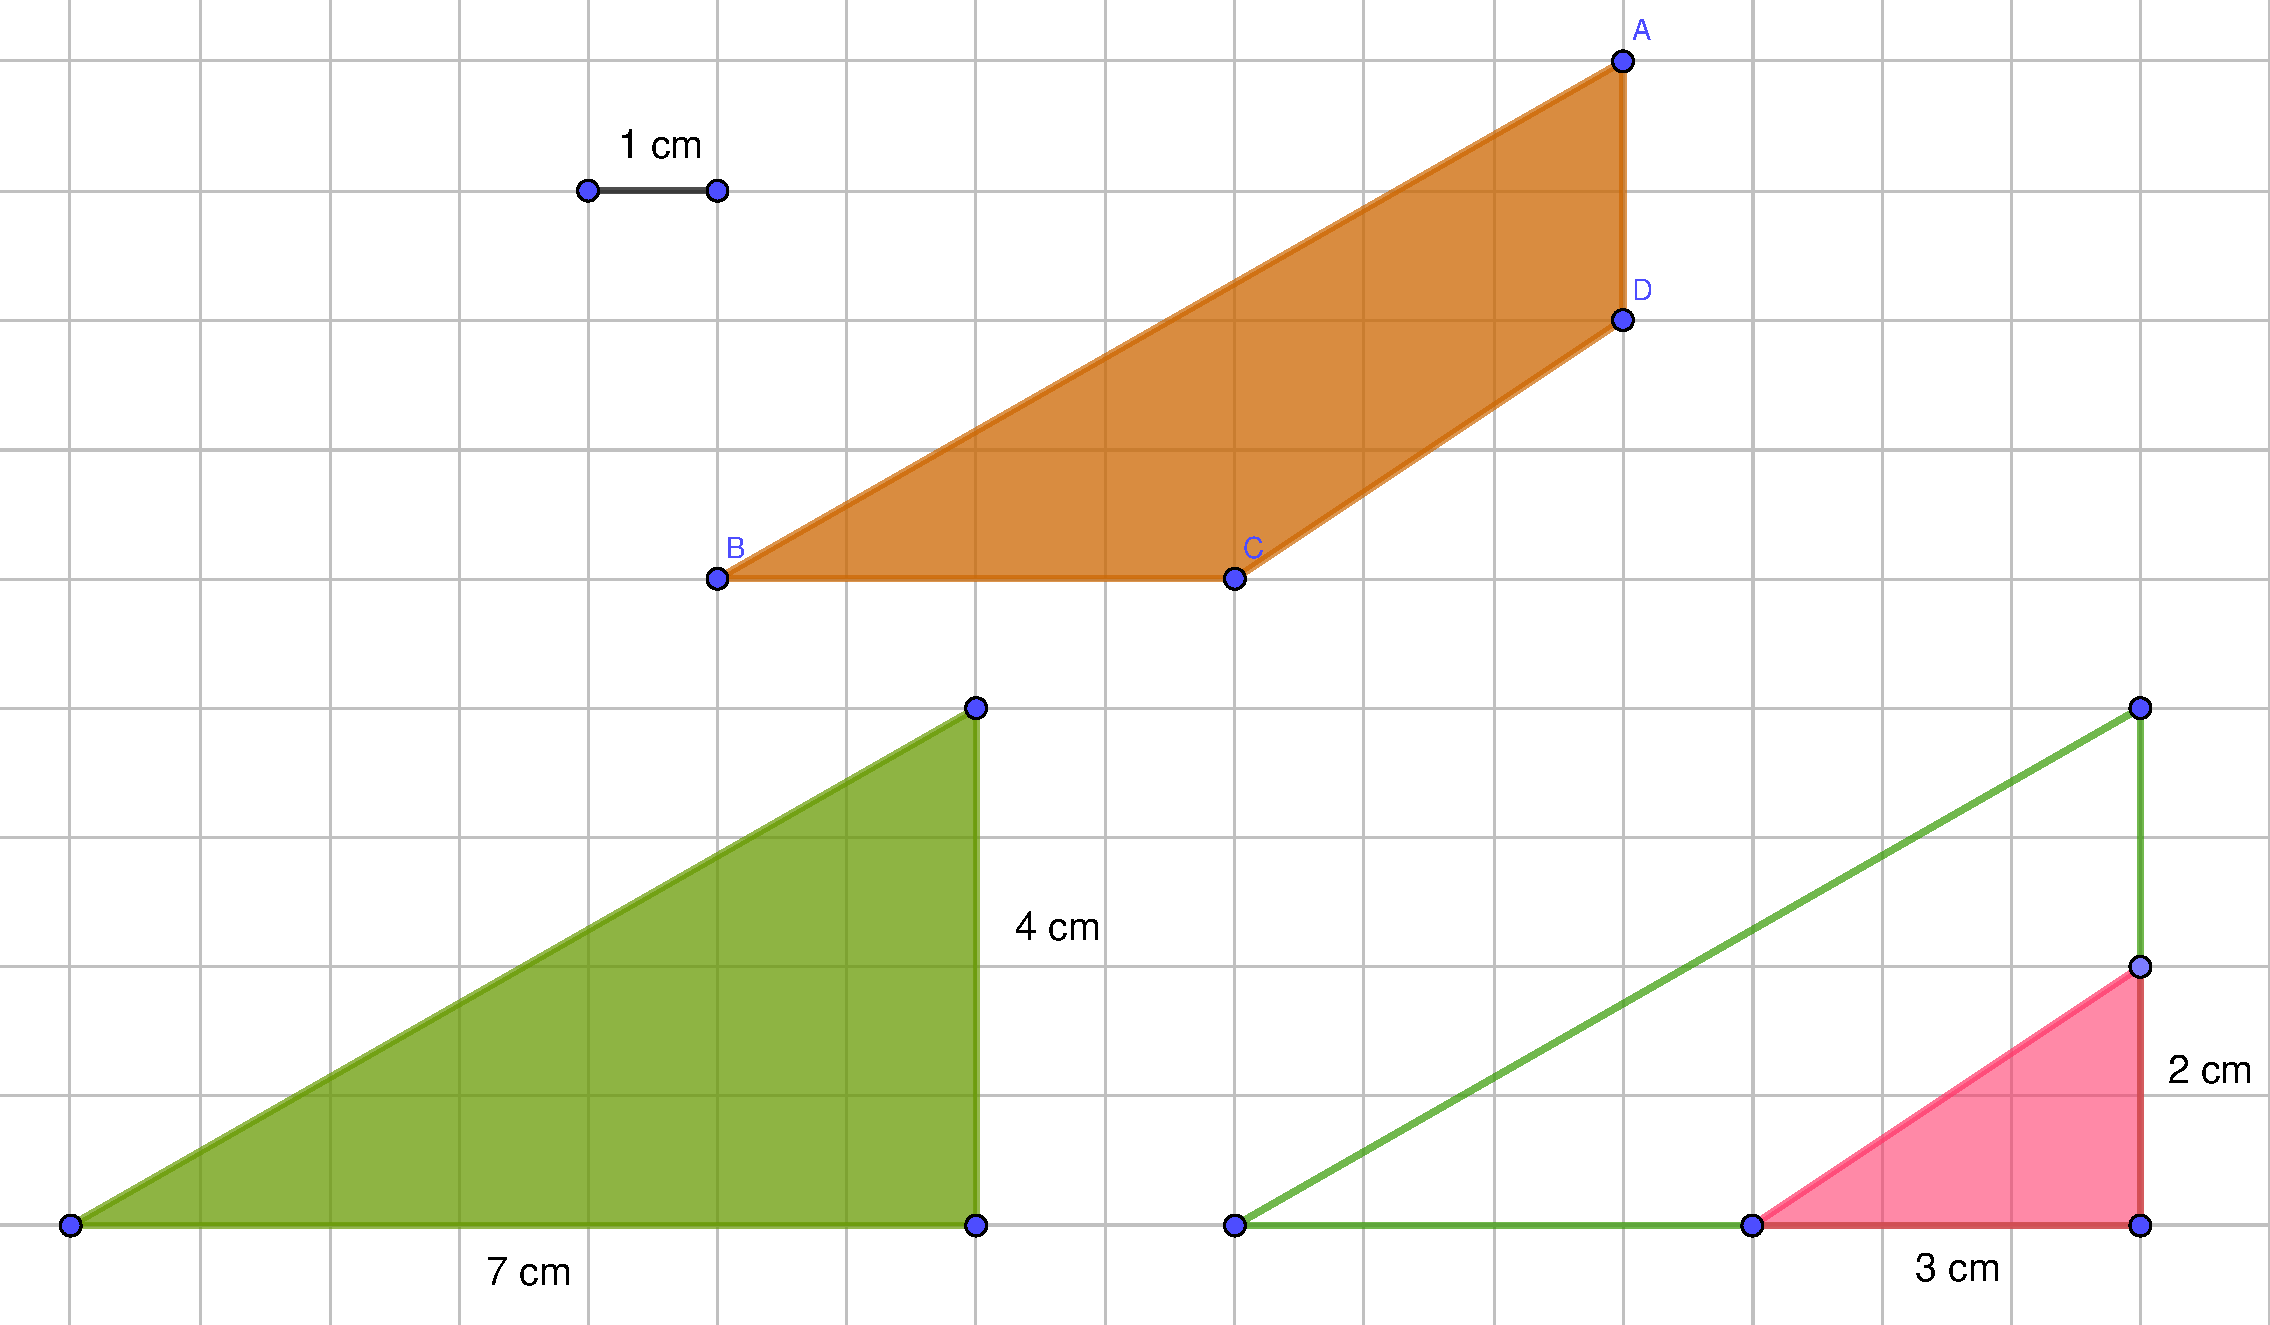
\includegraphics[width=0.6\textwidth]{teor/priklad-obsah}
    \end{center}
\end{minipage}

\subsection{Osová souměrnost}

Osová souměrnost je geometrické zobrazení. Při ní se každý bod útvaru zobrazí na druhou stranu nějaké předem určené osy, která se nazývá osa souměrnosti. Osa souměrnosti je určena přímkou.

Osová souměrnost se dá představit jako překlopení podle osy.

\subsubsection{Příklad}
\begin{minipage}[t]{\linewidth}
    Tyto dva trojúhelníky jsou osově souměrné, jelikož všechny jejich body jsou „překlopené” podle osy s.
    \begin{center}
        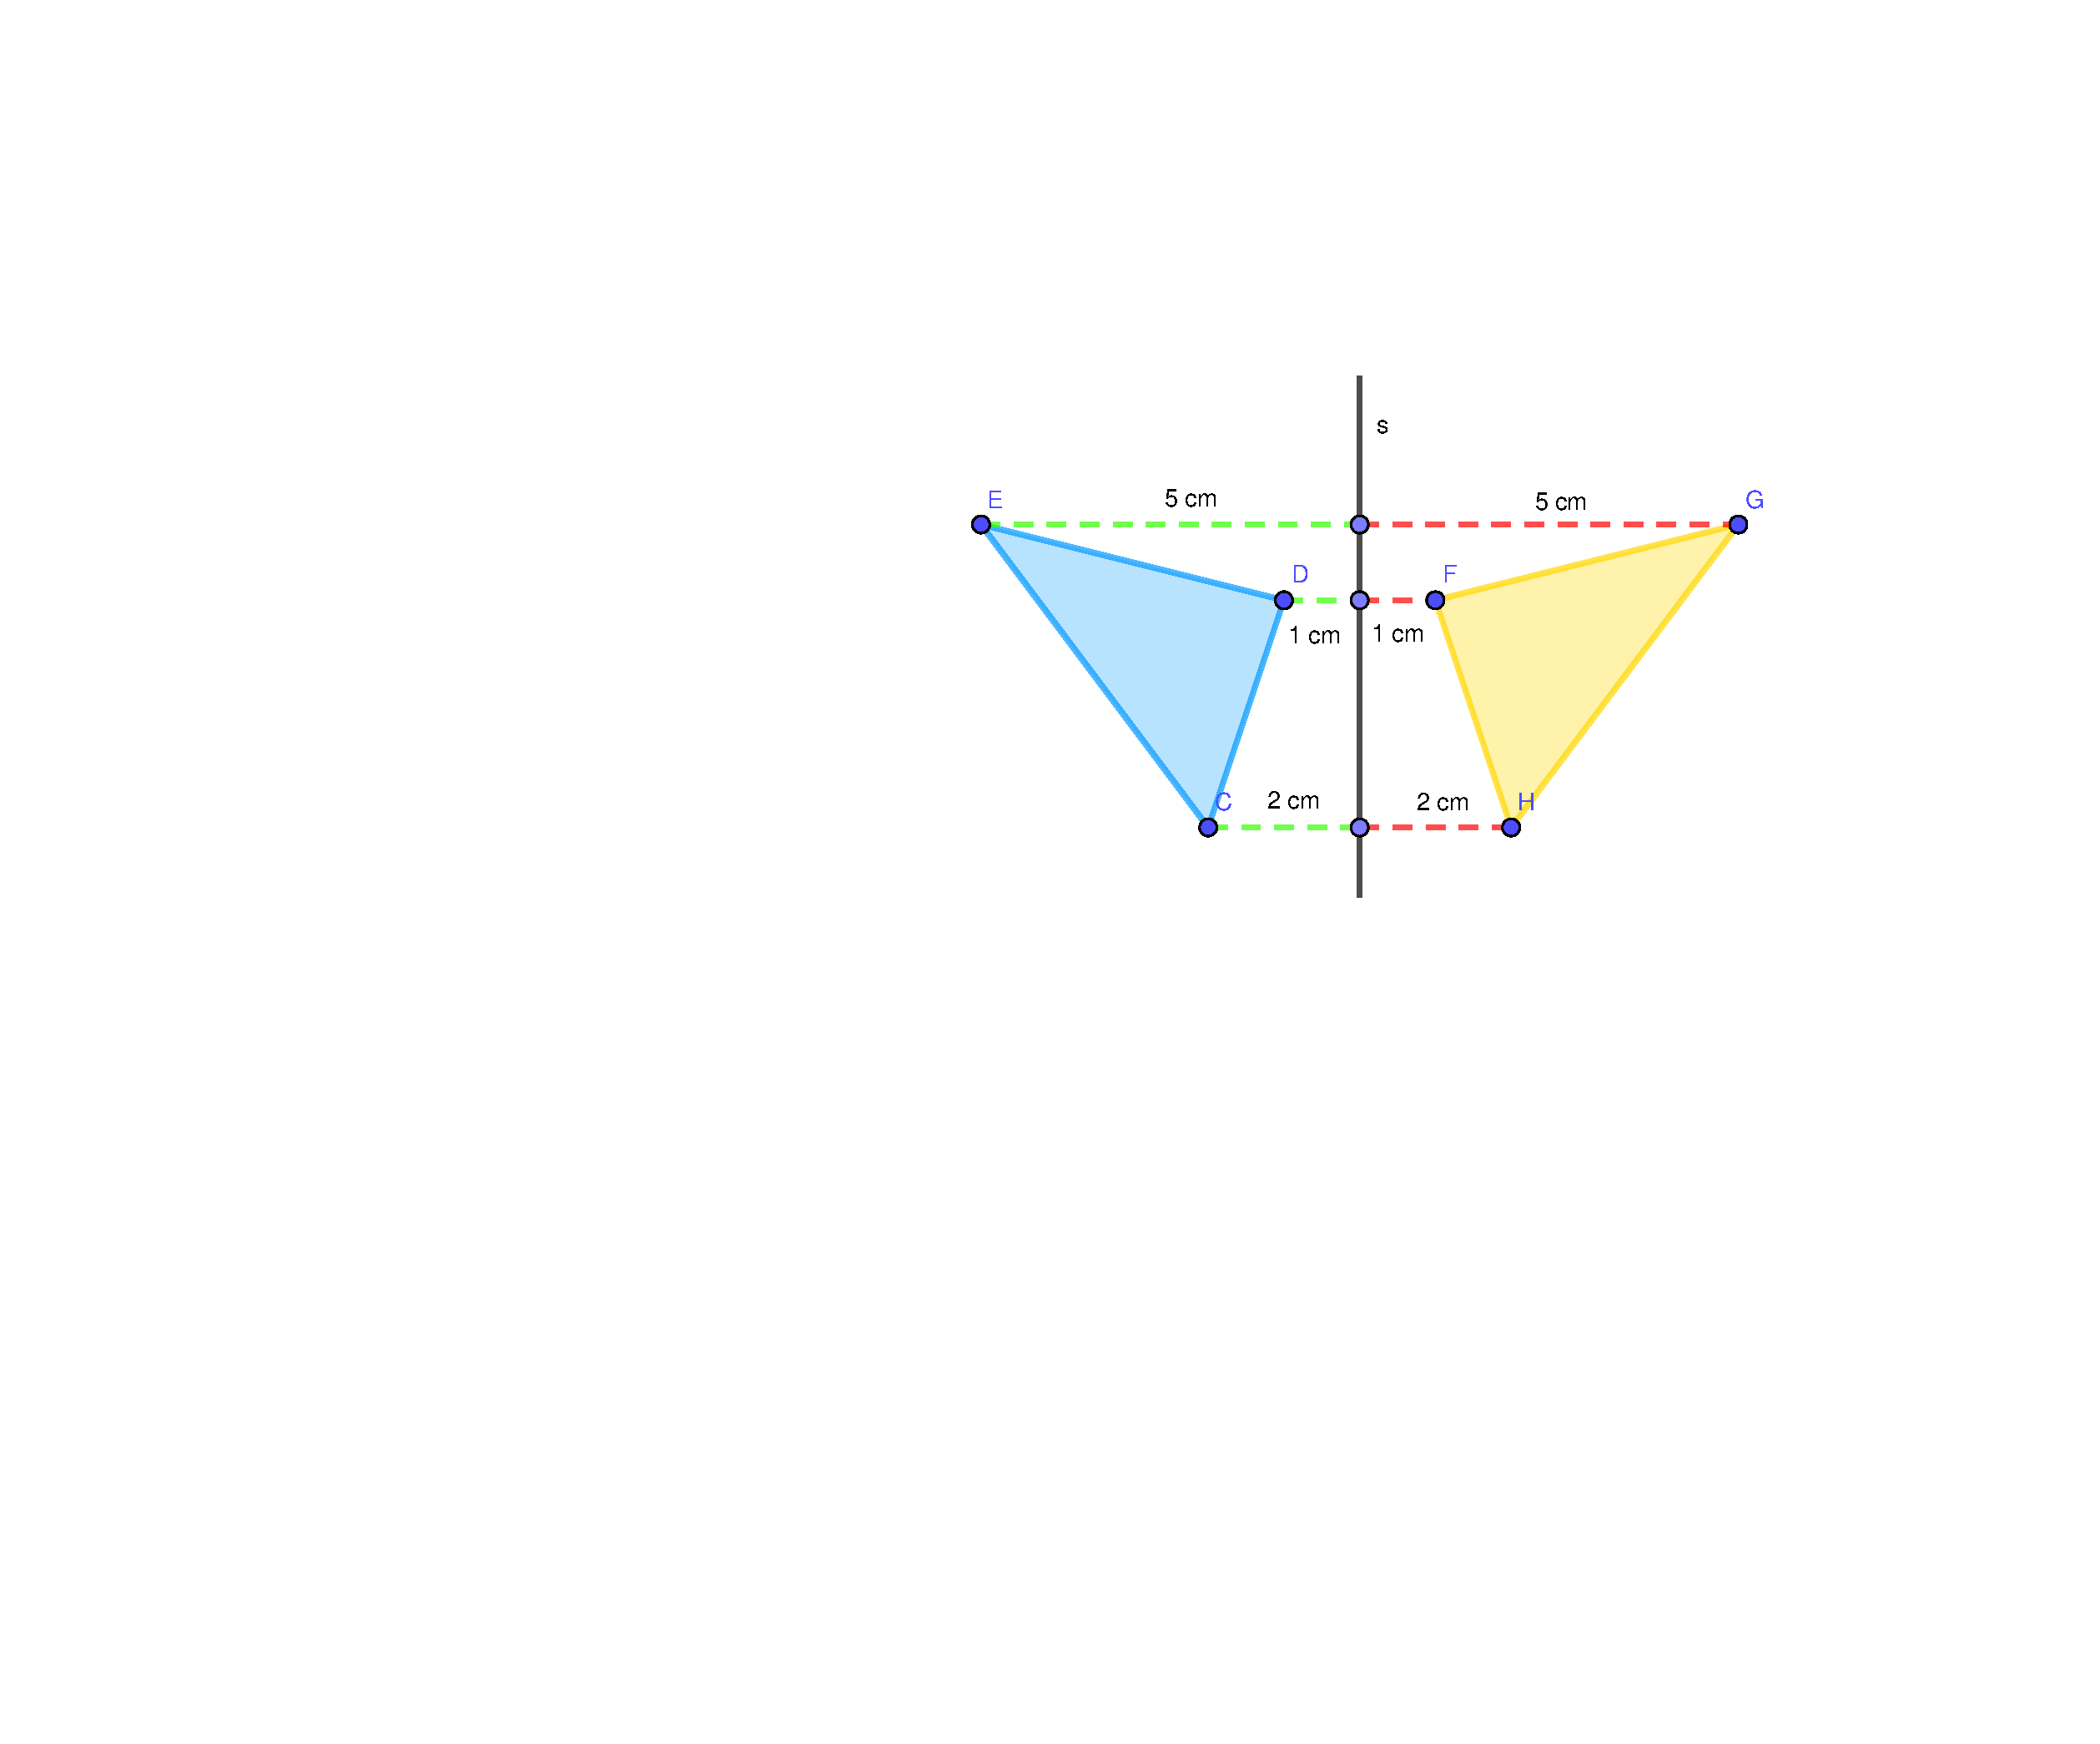
\includegraphics[width=0.6\textwidth]{teor/priklad-soum}
    \end{center}
\end{minipage}

\subsection{Rovnostranný trojúhelník}
Rovnostranný trojúhelník je trojúhelník, jehož všechny strany mají stejnou délku.

\begin{figure}[h]
    \centering
    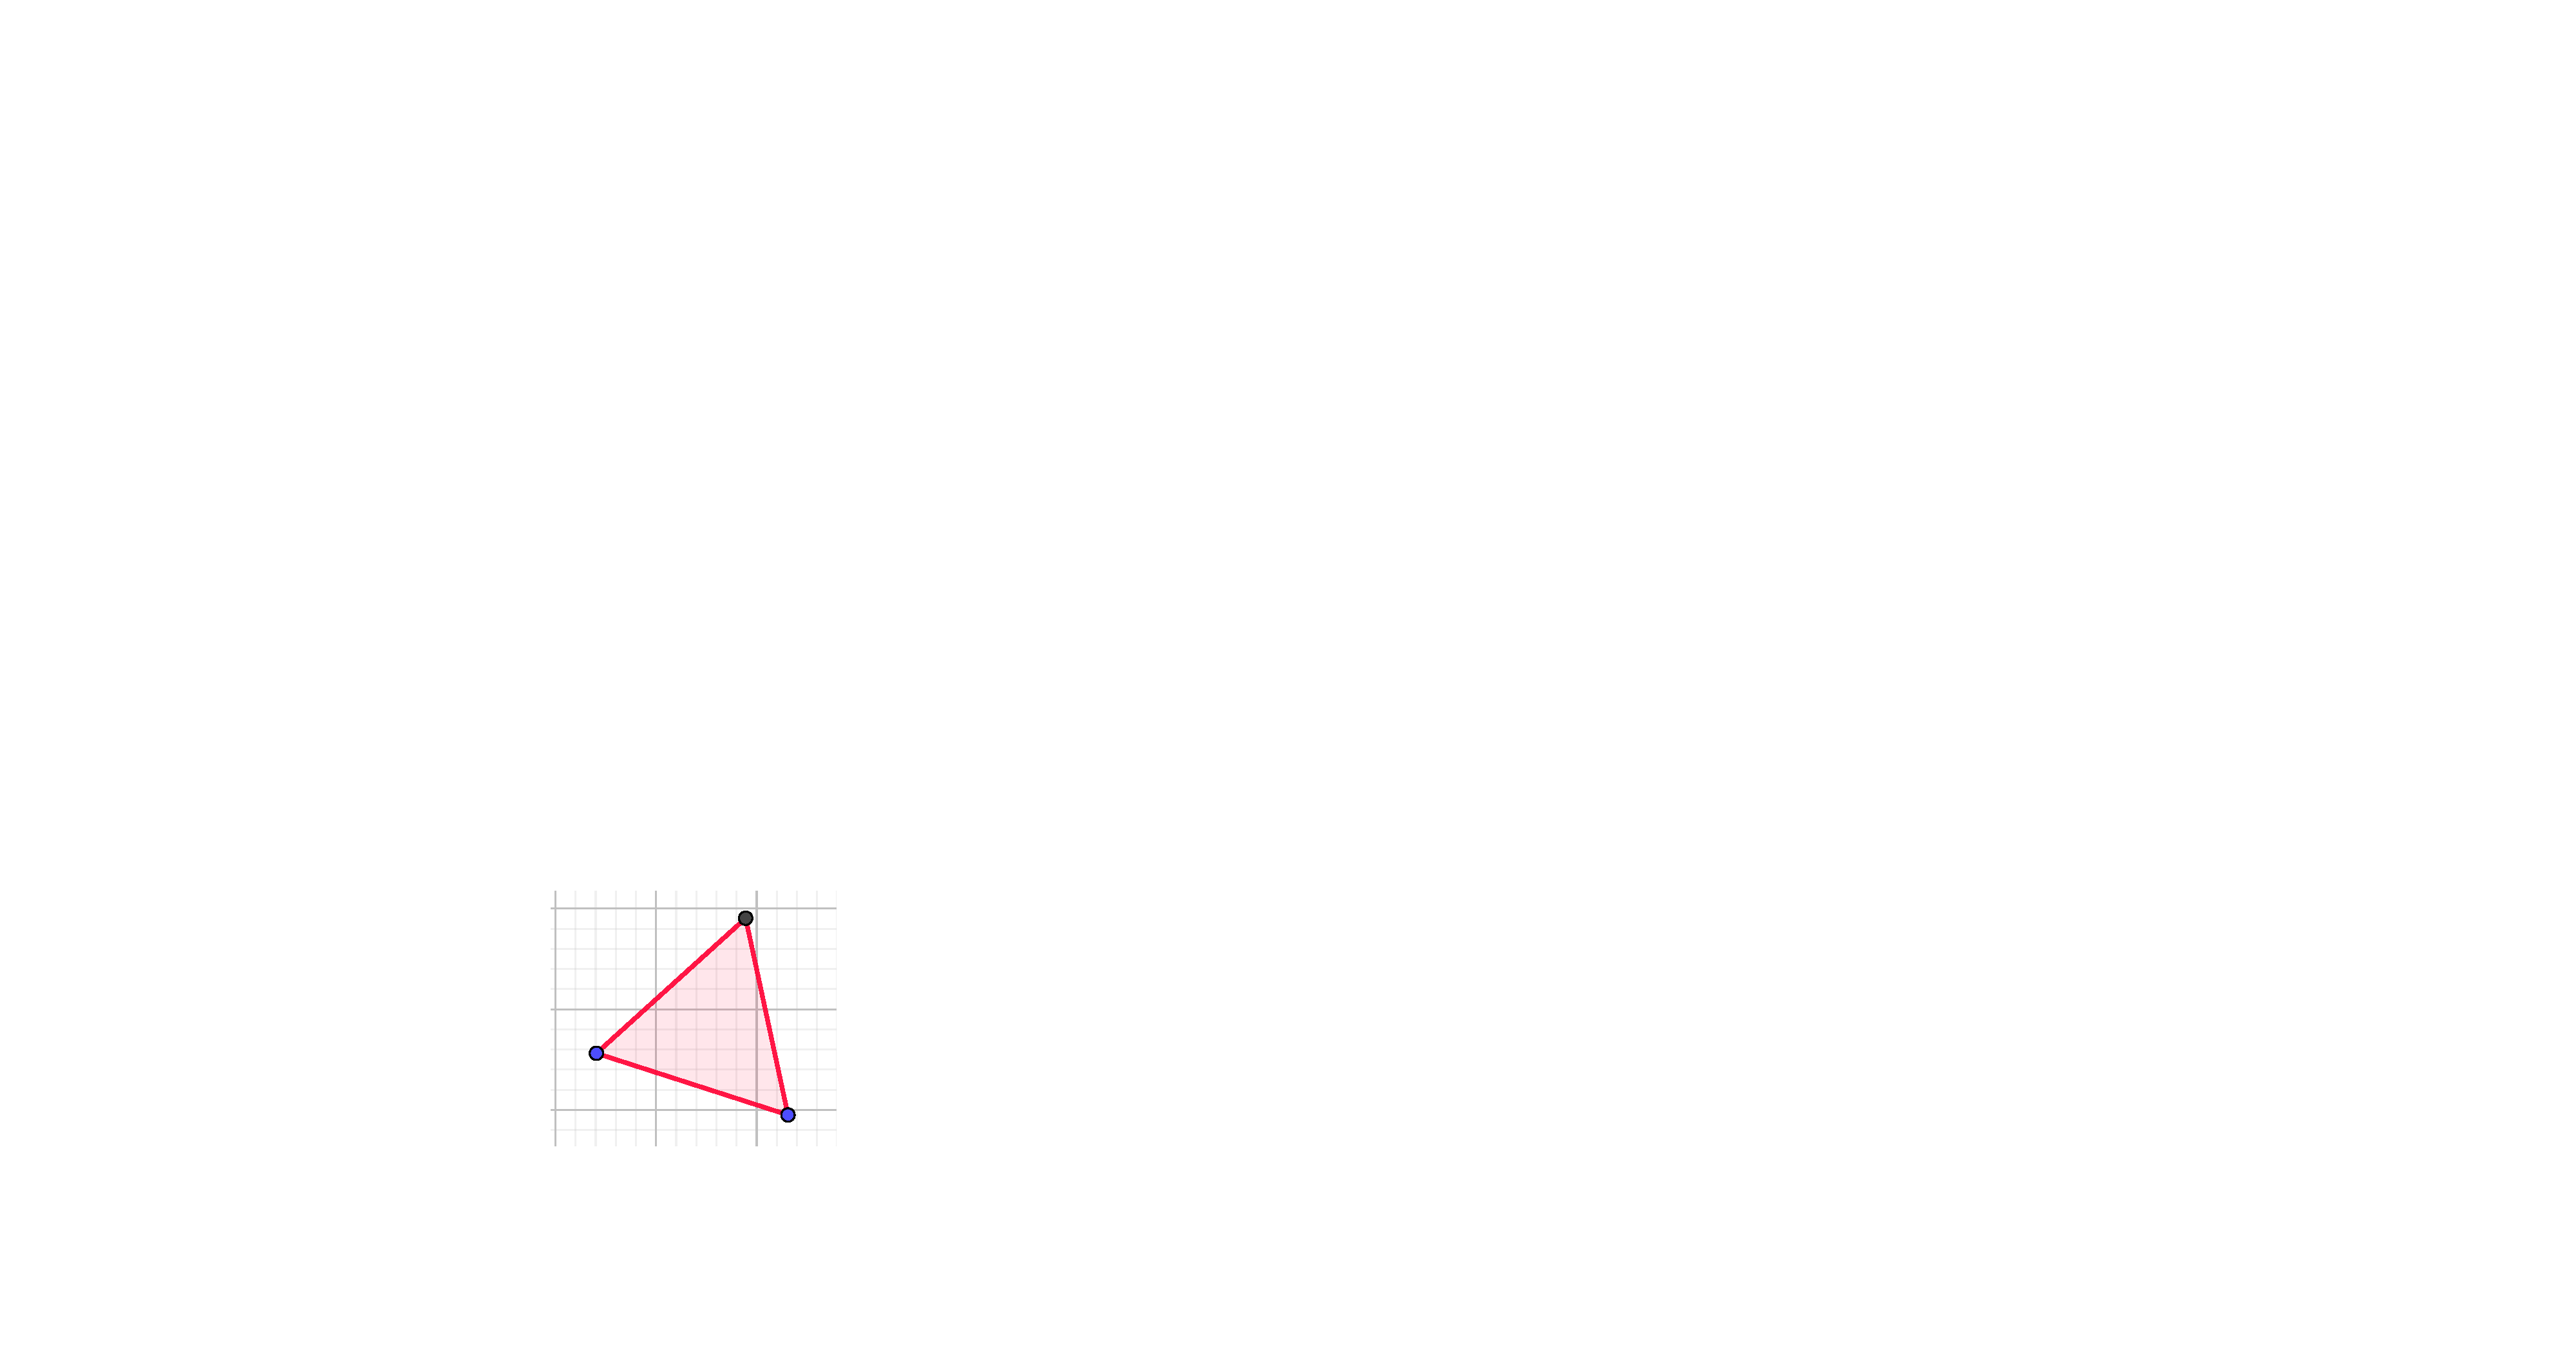
\includegraphics[width=0.3\textwidth]{teor/rovnostranny}
    \caption{Rovnostranný trojúhelník}
\end{figure}

\subsection{Rovnoramenný trojúhelník}
Rovnoramenný trojúhelník je trojúhelník, jehož dvě strany mají stejnou délku. Tyto dvě strany se nazývají ramena, třetí strana se jmenuje základna.

\begin{figure}[h]
    \centering
    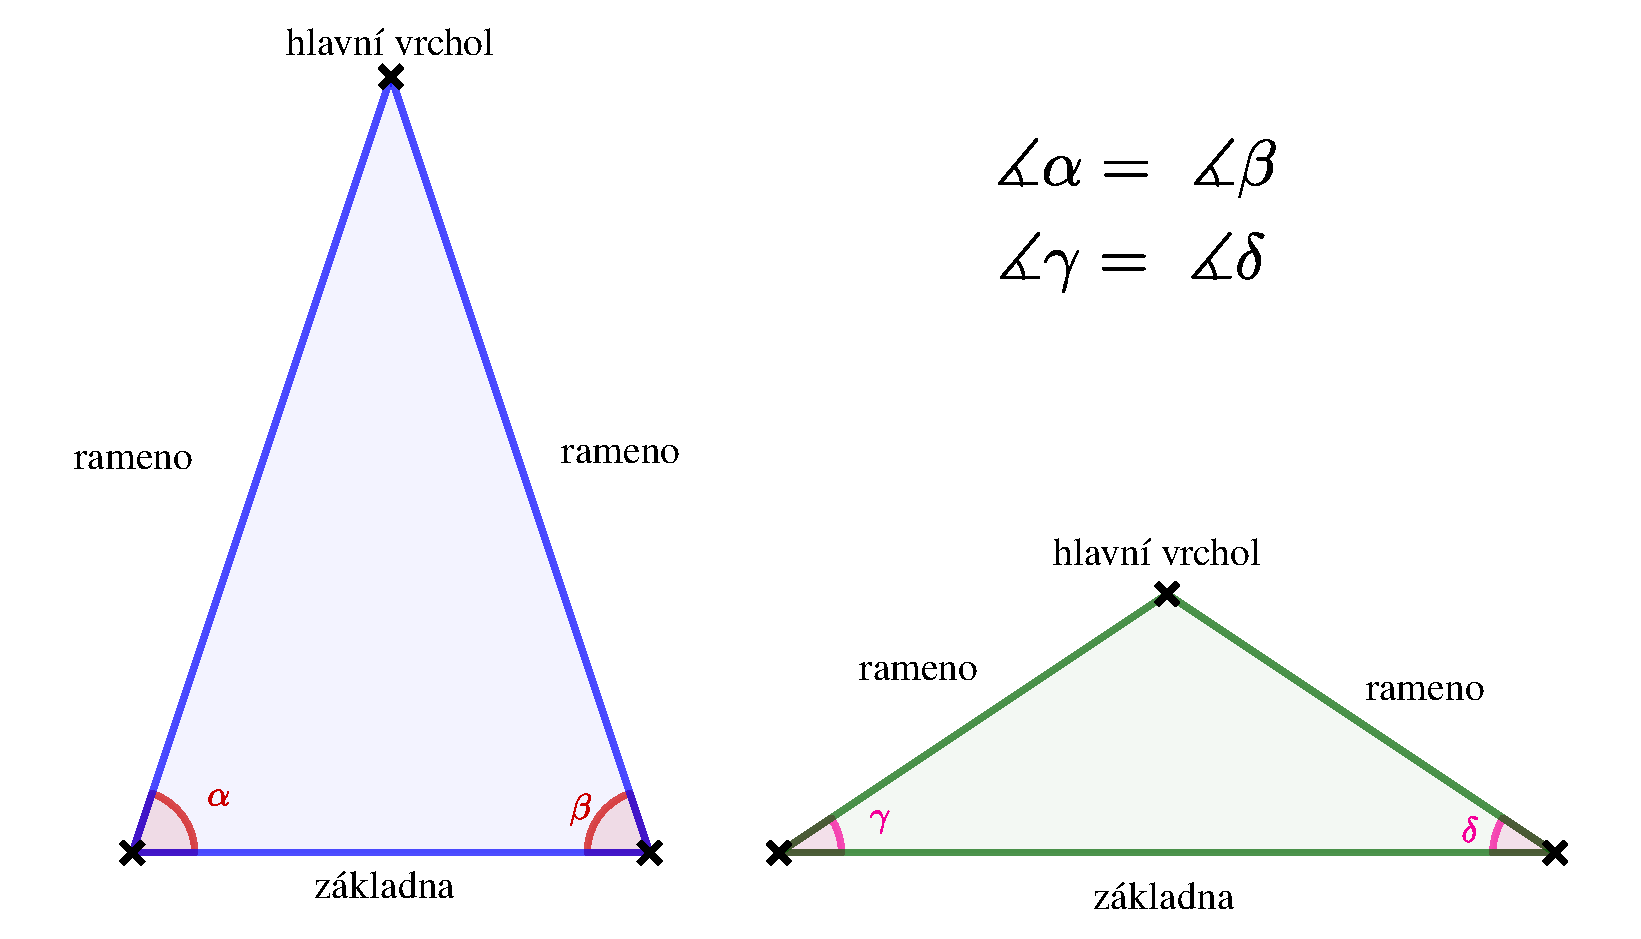
\includegraphics[width=0.6\textwidth]{teor/rovnoramenny}
    \caption{2 rovnoramenné trojúhelníky}
\end{figure}

\subsection{Shodnost trojúhelníků}
Dva trojúhelníky jsou navzájem shodné, pokud se rovnají délky všech jejich stran.

\subsection{Průsečík}
Průsečík je bod, ve kterém se protínají 2 čáry, například přímky nebo úsečky.

\begin{figure}[h]
    \centering
    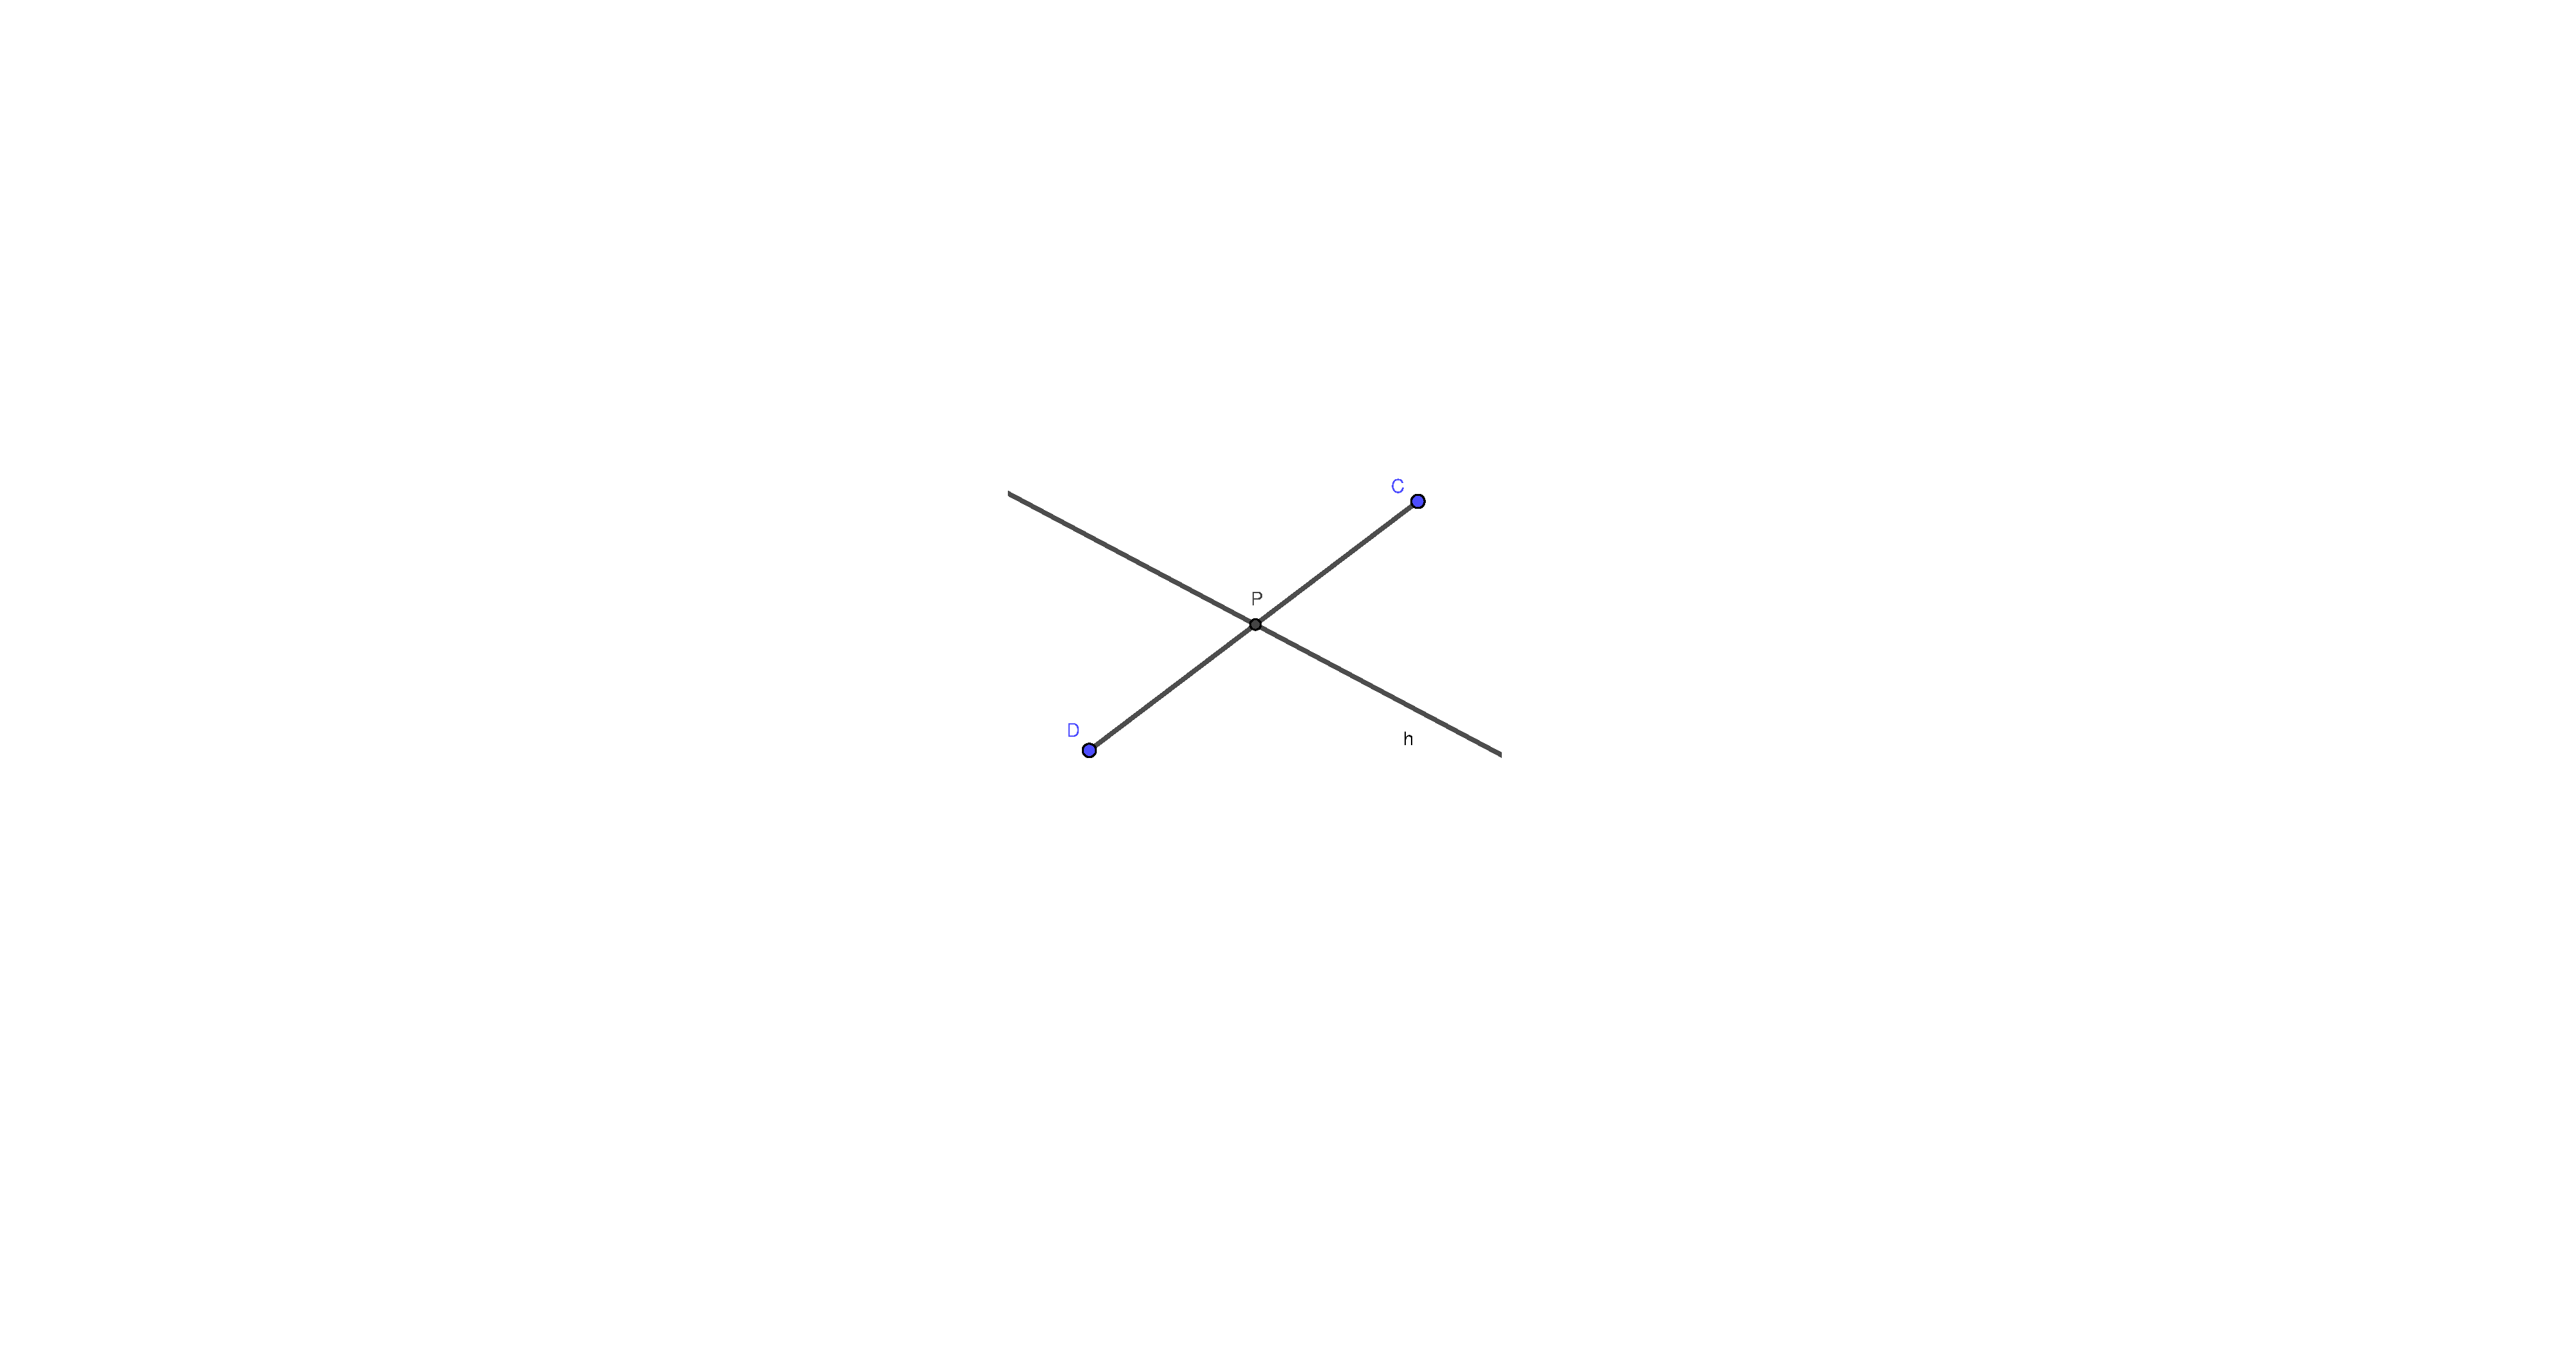
\includegraphics[width=0.6\textwidth]{teor/prusecik}
    \caption{Průsečík přímky h a úsečky CD, který je nazvaný P}
\end{figure}

\subsection{Pravý úhel, kolmost}
Pravý úhel je úhel o velikosti 90°. 2 čáry jsou na sebe kolmé, pokud svírají pravý úhel.

\begin{figure}[h]
    \centering
    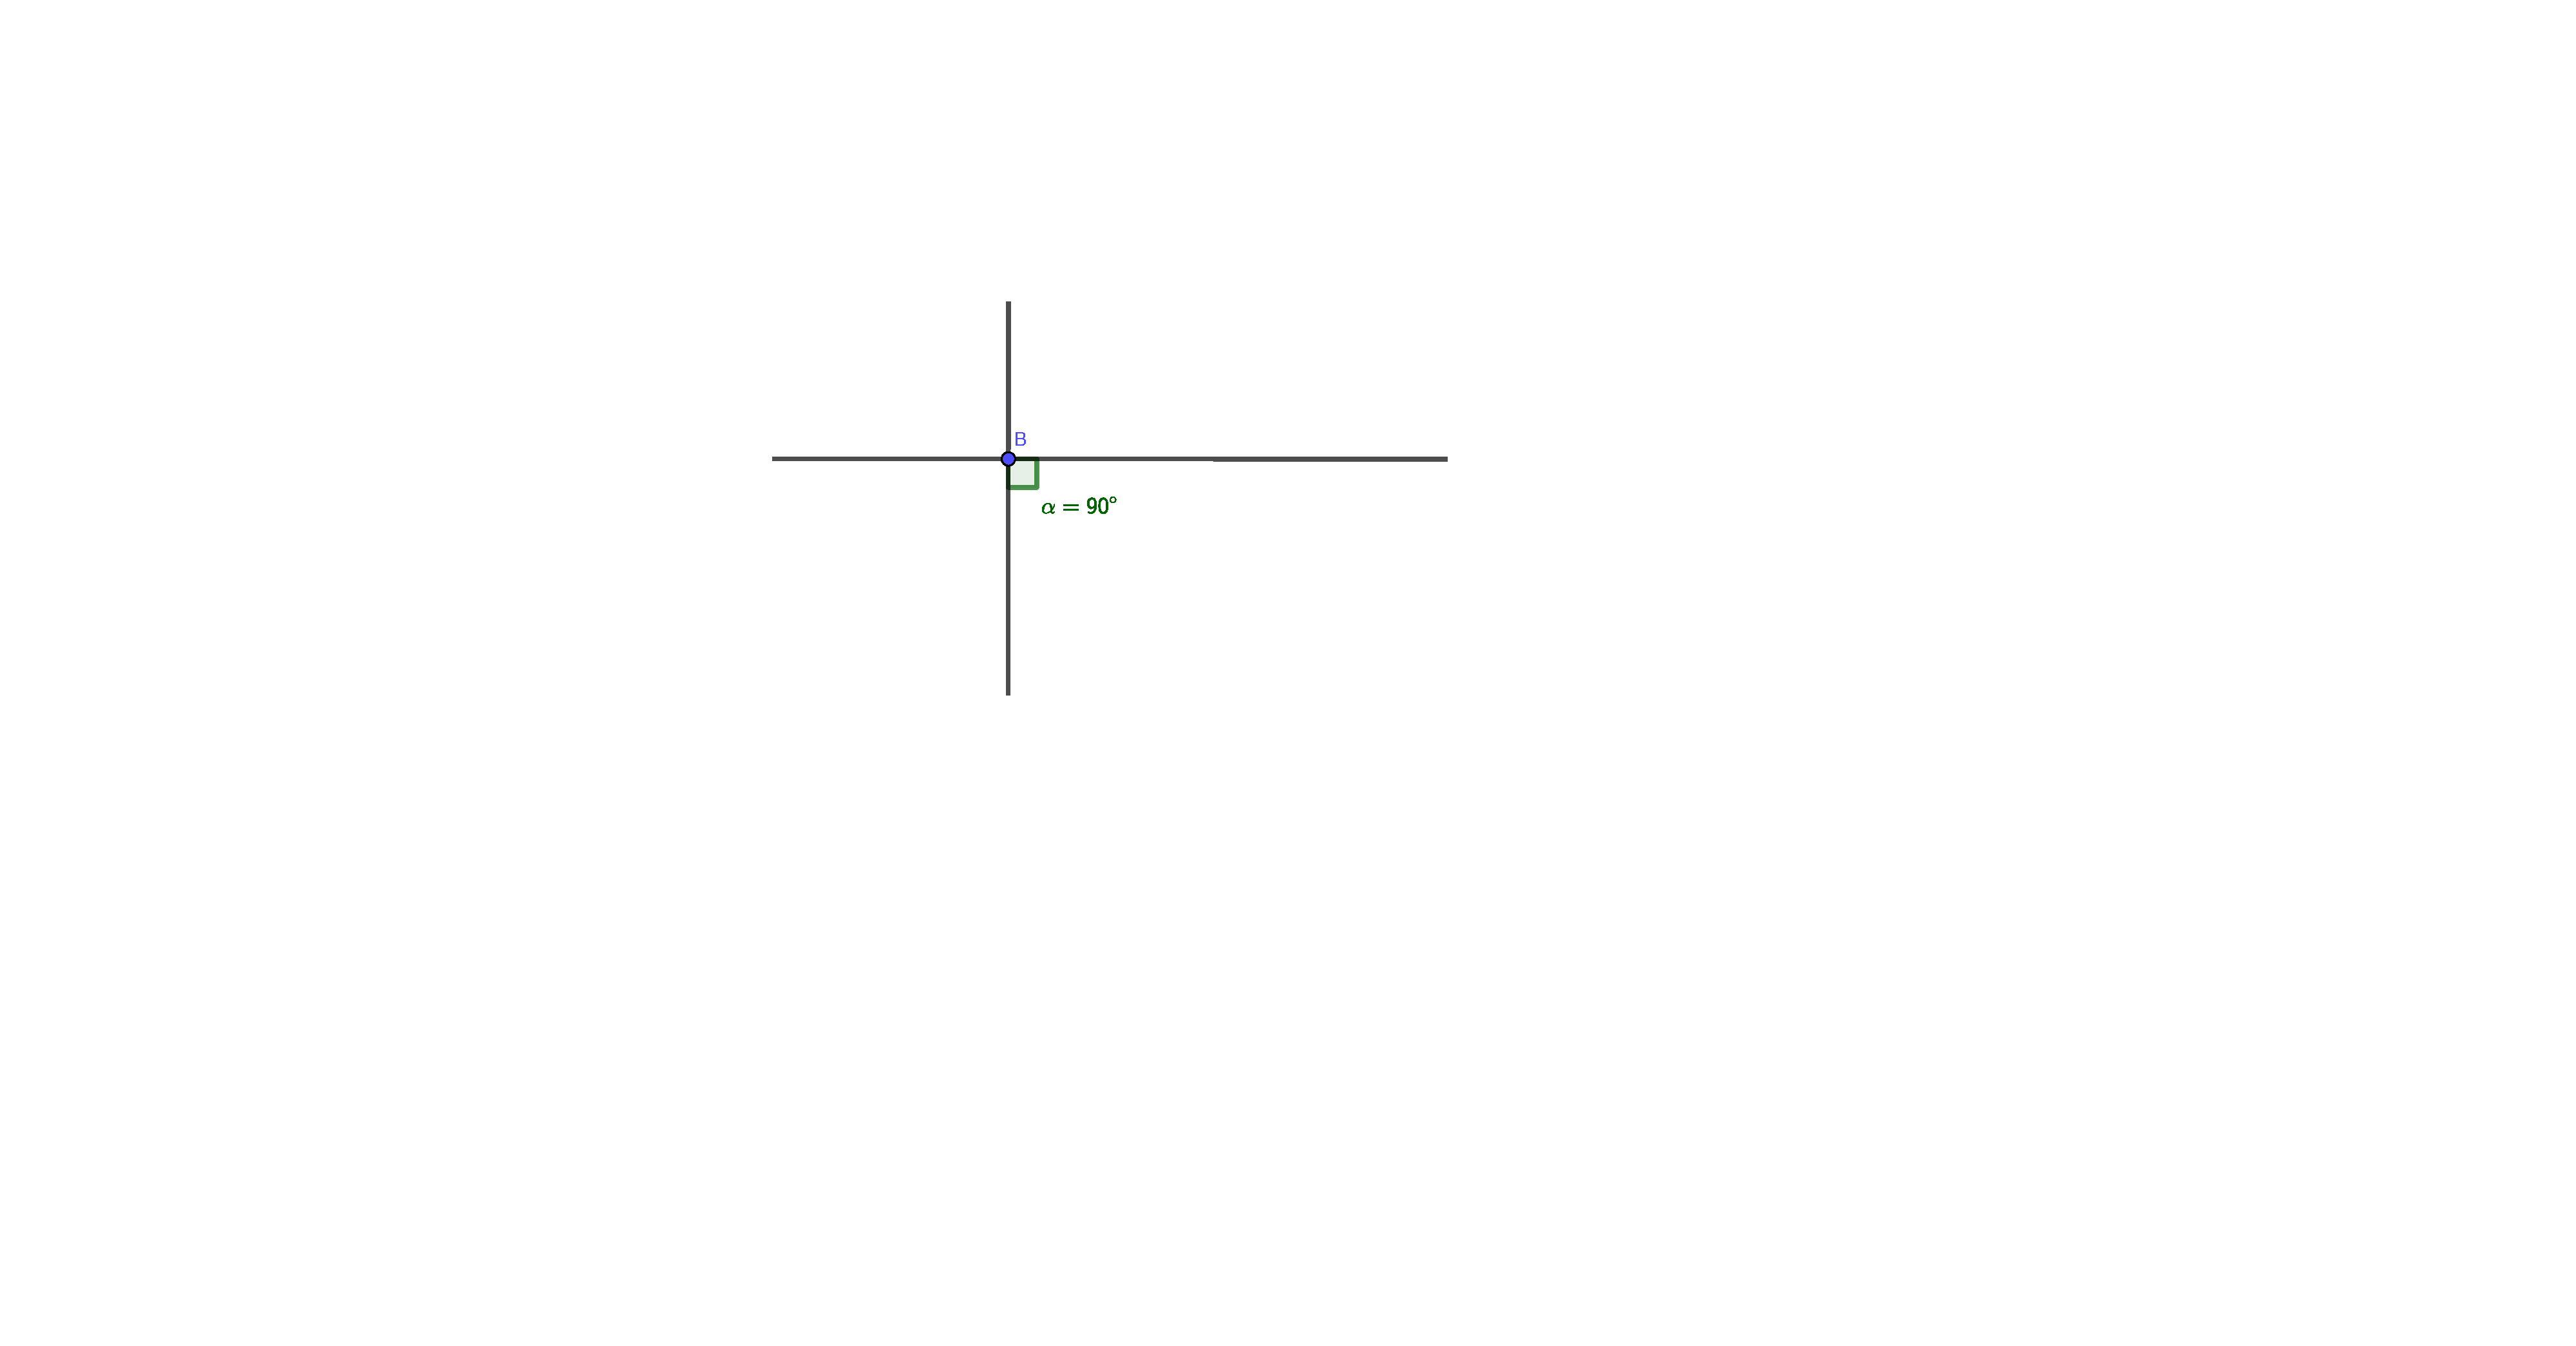
\includegraphics[width=0.4\textwidth]{teor/pravy-a-kolmo}
    \caption{Kolmice}
    \label{fig:kolm}
\end{figure}

Na obrázku~\ref{fig:kolm} jsou vidět 2 kolmé čáry svírající pravý úhel označený $\alpha$.

\subsection{Pravoúhlý trojúhelník}
Trojúhelník je pravoúhlý, pokud je jeden z jeho úhlů pravý.

\begin{figure}[h]
    \centering
    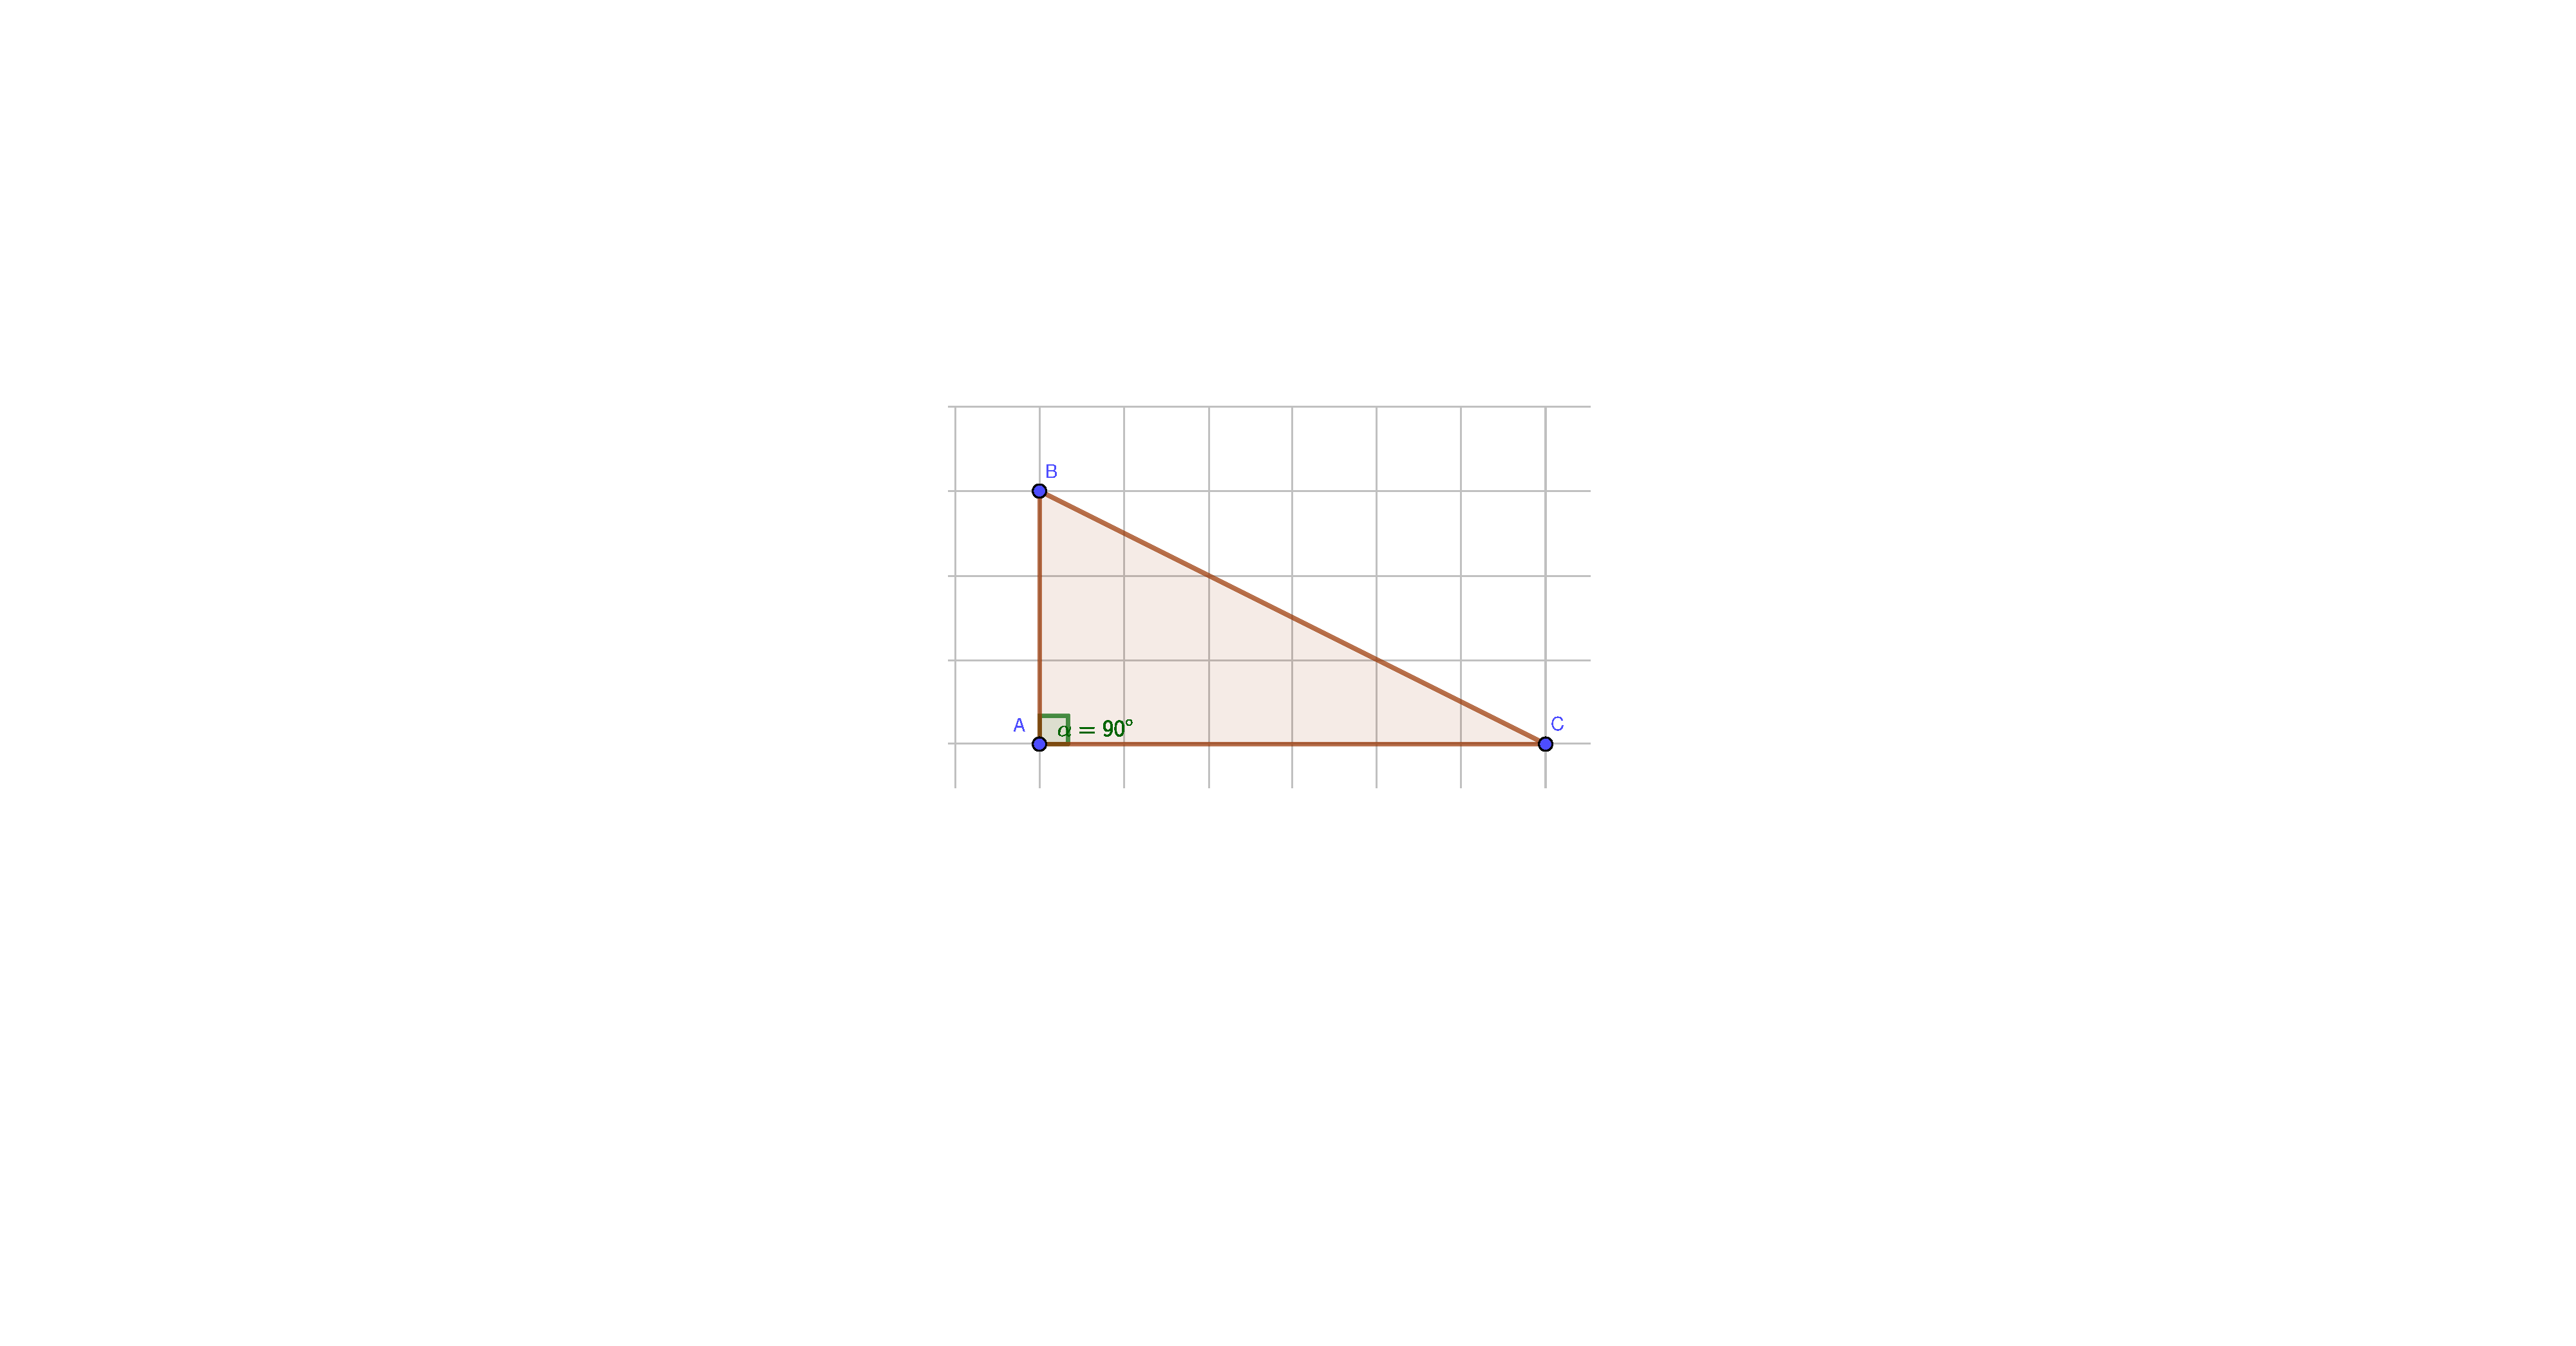
\includegraphics[width=0.6\textwidth]{teor/pravouhly}
    \caption{Pravoúhlý trojúhelník}
    \label{fig:pravouhly_troj}
\end{figure}

Na obrázku~\ref{fig:pravouhly_troj} je vidět pravoúhlý trojúhelník, jehož pravý úhel je označen $\alpha$.

\subsection{Rovnoběžnost}
Přímky jsou na sebe rovnoběžné, pokud se nikdy nepotkají. Úsečky jsou na sebe rovnoběžné, pokud se jimi vedené přímky nikdy nepotkají.

\begin{figure}[h]
    \centering
    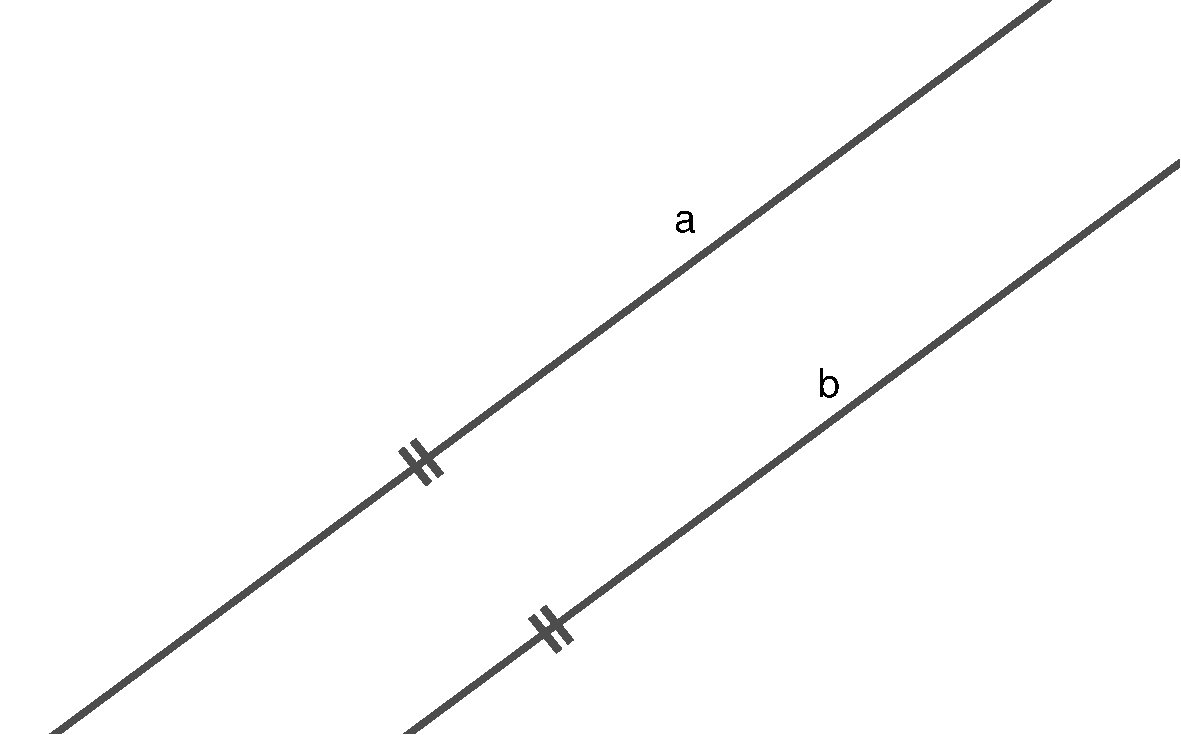
\includegraphics[width=0.6\textwidth]{teor/rovnobezky}
    \caption{2 rovnoběžné přímky}
\end{figure}

\subsection{Krychle}
Krychle je prostorové těleso. Také se nazývá kostka.

\subsubsection{Vrcholy}
Vrcholy krychle jsou body, které jsou v jejích rozích. Krychle jich má 8.

\subsubsection{Hrany}
Hrany jsou čáry, které spojují vrcholy. Krychle jich má 12.

\subsubsection{Stěny}
Stěny jsou čtverce tvořené 4 vrcholy krychle. Krychle jich má 6.

\subsubsection{Povrch}
Povrch krychle je součet obsahů jejích stěn, neboli 6krát obsah jedné stěny. Měří se v jednotkách obsahu.

Na obrázku~\ref{fig:krychle} je krychle, na které jsou červeně vyznačeny vrcholy, modře hrany a zeleně stěny.

\begin{figure}[h]
    \centering
    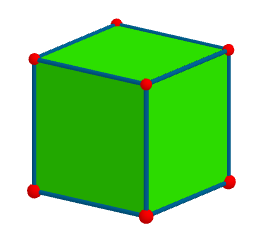
\includegraphics[width=0.6\textwidth]{teor/kostka}
    \caption{Krychle}
    \label{fig:krychle}
\end{figure}




    \chapter{Praktická část}


\section{Výběr úloh}

Nejdříve jsme získali přijímací zkoušky CERMAT od roku 2015 do roku 2022. Ty jsou volně dostupné na internetu. Z každého roku jsme se snažili čerpat z~pravých testů, tedy řádných a náhradních termínů, a ne ilustračních. Pokud ale v daný rok bylo pravých testů málo, použili jsme i ty.

Jako první jsme tyto zkoušky prošli, a vybrali z nich všechny úlohy které se týkají planimetrie nebo stereometrie.

Následovně jsme tyto úlohy kategorizovali podle
\begin{itemize}
    \item typu oboru,
    \item termínu ze kterého pochází
    \item a posledně do 3 hlavních kategorií, jimiž jsou
    \begin{itemize}
        \item úlohy planimetrické,
        \item stereometrické a
        \item rýsovací.
    \end{itemize}
\end{itemize}

V testech se neobjevily žádné stereometrické rýsovací úlohy, pouze planimetrické rýsovací.

Úloh jsme napříč vybrali 456.

Následně jsme všechny úlohy jednoho oboru dali k sobě podle kategorií a~vytvořili podkategorie. Například jedna z podkategorií planimetrických úloh pro 6leté obory byly úlohy zaměřené na úhly.


\section[Statistická analýza přijímacích zkoušek z minulých let]{Statistická analýza přijímacích zkoušek\\z minulých let}

Po roztřídění všech úloh jsme spočítali, jak často se v testech objevují a jakou mají bodovou váhu.

Přišli jsme k závěru že planimetrické a stereometrické úlohy jsou velmi důležité, jelikož v 8letých oborech odpovídají skoro 38 \% známky. Také se planimetrické, rýsovací a stereometrické úlohy objevují přibližně v poměru 2 : 1 : 1 pro tyto obory.

\begin{table}[htbp]
    \caption{Distribuce počtu úloh pro 8leté obory}
    \begin{tabular}{|l|l|r|r|r|r|}
        \hline
        \multicolumn{ 2}{|c|}{8leté obory} & \multicolumn{ 4}{c|}{Počet úloh} \\ \cline{ 3- 6}
        \multicolumn{ 2}{|l|}{} & \multicolumn{1}{c|}{Planimetrie} & \multicolumn{1}{c|}{\begin{tabular}[c]{@{}c@{}}
                                                                                             Rýsování\\ planimetrie
        \end{tabular}} & \multicolumn{1}{c|}{Stereometrie} & \multicolumn{1}{c|}{Celkem} \\ \hline
        \multicolumn{ 1}{|c|}{2022} & 1. řádný termín    & 2 & 1 & 1 & 14 \\ \cline{ 2- 6}
        \multicolumn{ 1}{|l|}{}     & 2. řádný termín    & 1 & 1 & 3 & 14 \\ \cline{ 2- 6}
        \multicolumn{ 1}{|l|}{}     & 1. náhradní termín & 4 & 1 & 1 & 14 \\ \cline{ 2- 6}
        \multicolumn{ 1}{|l|}{}     & 2. náhradní termín & 2 & 1 & 2 & 14 \\ \hline
        \multicolumn{ 1}{|c|}{2021} & 1. řádný termín    & 2 & 1 & 1 & 14 \\ \cline{ 2- 6}
        \multicolumn{ 1}{|l|}{}     & 2. řádný termín    & 2 & 1 & 1 & 14 \\ \cline{ 2- 6}
        \multicolumn{ 1}{|l|}{}     & 1. náhradní termín & 3 & 1 & 1 & 14 \\ \cline{ 2- 6}
        \multicolumn{ 1}{|l|}{}     & 2. náhradní termín & 2 & 1 & 1 & 14 \\ \hline
        \multicolumn{ 1}{|c|}{2020} & 1. řádný termín    & 2 & 1 & 1 & 14 \\ \cline{ 2- 6}
        \multicolumn{ 1}{|l|}{}     & 1. náhradní termín & 3 & 1 & 1 & 14 \\ \hline
        \multicolumn{ 1}{|c|}{2019} & 1. řádný termín    & 3 & 1 & 1 & 14 \\ \cline{ 2- 6}
        \multicolumn{ 1}{|l|}{}     & 2. řádný termín    & 3 & 1 & 1 & 14 \\ \cline{ 2- 6}
        \multicolumn{ 1}{|l|}{}     & 1. náhradní termín & 2 & 1 & 2 & 14 \\ \cline{ 2- 6}
        \multicolumn{ 1}{|l|}{}     & 2. náhradní termín & 1 & 1 & 2 & 14 \\ \hline
        \multicolumn{ 1}{|c|}{2018} & 1. řádný termín    & 1 & 1 & 1 & 14 \\ \cline{ 2- 6}
        \multicolumn{ 1}{|l|}{}     & 2. řádný termín    & 2 & 1 & 2 & 14 \\ \cline{ 2- 6}
        \multicolumn{ 1}{|l|}{}     & 1. náhradní termín & 1 & 1 & 2 & 14 \\ \cline{ 2- 6}
        \multicolumn{ 1}{|l|}{}     & 2. náhradní termín & 4 & 1 & 1 & 14 \\ \hline
        \multicolumn{ 1}{|c|}{2017} & 1. řádný termín    & 1 & 1 & 1 & 14 \\ \cline{ 2- 6}
        \multicolumn{ 1}{|l|}{}     & 2. řádný termín    & 3 & 1 & 1 & 14 \\ \cline{ 2- 6}
        \multicolumn{ 1}{|l|}{}     & 1. náhradní termín & 3 & 1 & 1 & 14 \\ \cline{ 2- 6}
        \multicolumn{ 1}{|l|}{}     & 2. náhradní termín & 3 & 1 & 1 & 14 \\ \hline
        \multicolumn{ 1}{|c|}{2016} & 1. řádný termín    & 3 & 1 & 2 & 16 \\ \cline{ 2- 6}
        \multicolumn{ 1}{|l|}{}     & Ilustrační         & 3 & 1 & 2 & 16 \\ \hline
        \multicolumn{ 1}{|c|}{2015} & 1. řádný termín    & 2 & 1 & 2 & 16 \\ \cline{ 2- 6}
        \multicolumn{ 1}{|l|}{}     & Ilustrační         & 2 & 2 & 1 & 17 \\ \hline
        \multicolumn{ 2}{|c|}{Průměr} & 2,31 & 1,04 & 1,38 & 14,35 \\ \hline
        \multicolumn{ 2}{|c|}{Průměrná četnost} & 16,09 \% & 7,24 \% & 9,65 \% & 32,98 \% \\ \hline
    \end{tabular}
    \label{tabulka8-1}
\end{table}

\begin{table}[htbp]
    \caption{Distribuce bodů za úlohu pro 8leté obory}
    \begin{tabular}{|l|l|r|r|r|r|}
        \hline
        \multicolumn{ 2}{|c|}{8leté obory} & \multicolumn{ 4}{c|}{Body za úlohy} \\ \cline{ 3- 6}
        \multicolumn{ 2}{|l|}{} & \multicolumn{1}{c|}{Planimetrie} & \multicolumn{1}{c|}{\begin{tabular}[c]{@{}c@{}}
                                                                                             Rýsování\\ planimetrie
        \end{tabular}} & \multicolumn{1}{c|}{Stereometrie} & \multicolumn{1}{c|}{Celkem} \\ \hline
        \multicolumn{ 1}{|c|}{2022} & 1. řádný termín    & 8  & 6 & 5 & 50 \\ \cline{ 2- 6}
        \multicolumn{ 1}{|l|}{}     & 2. řádný termín    & 2  & 6 & 7 & 50 \\ \cline{ 2- 6}
        \multicolumn{ 1}{|l|}{}     & 1. náhradní termín & 10 & 6 & 5 & 50 \\ \cline{ 2- 6}
        \multicolumn{ 1}{|l|}{}     & 2. náhradní termín & 12 & 6 & 4 & 50 \\ \hline
        \multicolumn{ 1}{|c|}{2021} & 1. řádný termín    & 8  & 6 & 5 & 50 \\ \cline{ 2- 6}
        \multicolumn{ 1}{|l|}{}     & 2. řádný termín    & 6  & 6 & 5 & 50 \\ \cline{ 2- 6}
        \multicolumn{ 1}{|l|}{}     & 1. náhradní termín & 10 & 6 & 5 & 50 \\ \cline{ 2- 6}
        \multicolumn{ 1}{|l|}{}     & 2. náhradní termín & 8  & 6 & 2 & 50 \\ \hline
        \multicolumn{ 1}{|c|}{2020} & 1. řádný termín    & 8  & 6 & 5 & 50 \\ \cline{ 2- 6}
        \multicolumn{ 1}{|l|}{}     & 1. náhradní termín & 12 & 6 & 4 & 50 \\ \hline
        \multicolumn{ 1}{|c|}{2019} & 1. řádný termín    & 12 & 6 & 5 & 50 \\ \cline{ 2- 6}
        \multicolumn{ 1}{|l|}{}     & 2. řádný termín    & 12 & 6 & 5 & 50 \\ \cline{ 2- 6}
        \multicolumn{ 1}{|l|}{}     & 1. náhradní termín & 8  & 6 & 4 & 50 \\ \cline{ 2- 6}
        \multicolumn{ 1}{|l|}{}     & 2. náhradní termín & 4  & 6 & 4 & 50 \\ \hline
        \multicolumn{ 1}{|c|}{2018} & 1. řádný termín    & 4  & 6 & 5 & 50 \\ \cline{ 2- 6}
        \multicolumn{ 1}{|l|}{}     & 2. řádný termín    & 8  & 6 & 4 & 50 \\ \cline{ 2- 6}
        \multicolumn{ 1}{|l|}{}     & 1. náhradní termín & 4  & 6 & 4 & 50 \\ \cline{ 2- 6}
        \multicolumn{ 1}{|l|}{}     & 2. náhradní termín & 12 & 6 & 2 & 50 \\ \hline
        \multicolumn{ 1}{|c|}{2017} & 1. řádný termín    & 4  & 6 & 5 & 50 \\ \cline{ 2- 6}
        \multicolumn{ 1}{|l|}{}     & 2. řádný termín    & 8  & 6 & 5 & 50 \\ \cline{ 2- 6}
        \multicolumn{ 1}{|l|}{}     & 1. náhradní termín & 11 & 6 & 2 & 50 \\ \cline{ 2- 6}
        \multicolumn{ 1}{|l|}{}     & 2. náhradní termín & 11 & 6 & 2 & 50 \\ \hline
        \multicolumn{ 1}{|c|}{2016} & 1. řádný termín    & 10 & 6 & 4 & 50 \\ \cline{ 2- 6}
        \multicolumn{ 1}{|l|}{}     & Ilustrační         & 10 & 6 & 4 & 50 \\ \hline
        \multicolumn{ 1}{|c|}{2015} & 1. řádný termín    & 6  & 6 & 4 & 50 \\ \cline{ 2- 6}
        \multicolumn{ 1}{|l|}{}     & Ilustrační         & 6  & 8 & 6 & 50 \\ \hline
        \multicolumn{ 2}{|c|}{Průměr} & 8,23 & 6,08 & 4,31 & 50,00 \\ \hline
        \multicolumn{ 2}{|c|}{\begin{tabular}[c]{@{}c@{}}
                                  Průměrná\\ četnost
        \end{tabular}} & 16,46 \% & 12,15 \% & 8,62 \% & 37,23 \% \\ \hline
    \end{tabular}
    \label{tabulka8-2}
\end{table}


\begin{table}[htbp]
    \caption{Distribuce počtu úloh pro 6leté obory}
    \begin{tabular}{|l|l|r|r|r|r|}
        \hline
        \multicolumn{ 2}{|l|}{6leté obory} & \multicolumn{ 3}{c|}{Počet úloh co obsahuje} & \multicolumn{ 1}{c|}{Celkem} \\ \cline{ 3- 5}
        \multicolumn{ 2}{|l|}{} & \multicolumn{1}{c|}{Planimetrie} & \multicolumn{1}{c|}{\begin{tabular}[c]{@{}c@{}}
                                                                                             Rýsování\\ planimetrie
        \end{tabular}} & \multicolumn{1}{c|}{Stereometrie} & \multicolumn{ 1}{c|}{} \\ \hline
        \multicolumn{ 1}{|c|}{2022} & 1. řádný termín    & 4 & 2 & 0 & 16 \\ \cline{ 2- 6}
        \multicolumn{ 1}{|l|}{}     & 2. řádný termín    & 4 & 2 & 1 & 16 \\ \cline{ 2- 6}
        \multicolumn{ 1}{|l|}{}     & 1. náhradní termín & 6 & 2 & 0 & 16 \\ \cline{ 2- 6}
        \multicolumn{ 1}{|l|}{}     & 2. náhradní termín & 3 & 2 & 1 & 16 \\ \hline
        \multicolumn{ 1}{|c|}{2021} & 1. řádný termín    & 3 & 2 & 1 & 16 \\ \cline{ 2- 6}
        \multicolumn{ 1}{|l|}{}     & 2. řádný termín    & 2 & 2 & 2 & 16 \\ \cline{ 2- 6}
        \multicolumn{ 1}{|l|}{}     & 1. náhradní termín & 4 & 2 & 1 & 16 \\ \cline{ 2- 6}
        \multicolumn{ 1}{|l|}{}     & 2. náhradní termín & 4 & 2 & 1 & 16 \\ \hline
        \multicolumn{ 1}{|c|}{2020} & 1. řádný termín    & 3 & 2 & 1 & 16 \\ \cline{ 2- 6}
        \multicolumn{ 1}{|l|}{}     & 1. náhradní termín & 3 & 2 & 1 & 16 \\ \hline
        \multicolumn{ 1}{|c|}{2019} & 1. řádný termín    & 3 & 2 & 1 & 16 \\ \cline{ 2- 6}
        \multicolumn{ 1}{|l|}{}     & 2. řádný termín    & 3 & 2 & 1 & 16 \\ \cline{ 2- 6}
        \multicolumn{ 1}{|l|}{}     & 1. náhradní termín & 5 & 2 & 0 & 16 \\ \cline{ 2- 6}
        \multicolumn{ 1}{|l|}{}     & 2. náhradní termín & 3 & 1 & 1 & 16 \\ \hline
        \multicolumn{ 1}{|c|}{2018} & 1. řádný termín    & 3 & 2 & 0 & 16 \\ \cline{ 2- 6}
        \multicolumn{ 1}{|l|}{}     & 2. řádný termín    & 3 & 2 & 1 & 16 \\ \cline{ 2- 6}
        \multicolumn{ 1}{|l|}{}     & 1. náhradní termín & 3 & 2 & 0 & 16 \\ \cline{ 2- 6}
        \multicolumn{ 1}{|l|}{}     & 2. náhradní termín & 3 & 2 & 1 & 16 \\ \hline
        \multicolumn{ 1}{|c|}{2017} & 1. řádný termín    & 3 & 2 & 1 & 17 \\ \cline{ 2- 6}
        \multicolumn{ 1}{|l|}{}     & 2. řádný termín    & 4 & 2 & 1 & 17 \\ \cline{ 2- 6}
        \multicolumn{ 1}{|l|}{}     & 1. náhradní termín & 4 & 2 & 2 & 17 \\ \cline{ 2- 6}
        \multicolumn{ 1}{|l|}{}     & 2. náhradní termín & 4 & 2 & 0 & 17 \\ \hline
        \multicolumn{ 1}{|c|}{2016} & 1. řádný termín    & 3 & 1 & 1 & 17 \\ \cline{ 2- 6}
        \multicolumn{ 1}{|l|}{}     & Ilustrační         & 4 & 1 & 1 & 17 \\ \hline
        \multicolumn{ 1}{|c|}{2015} & 1. řádný termín    & 3 & 1 & 1 & 17 \\ \cline{ 2- 6}
        \multicolumn{ 1}{|l|}{}     & Ilustrační         & 2 & 2 & 2 & 17 \\ \hline
        \multicolumn{ 2}{|c|}{Průměr} & 3,42 & 1,85 & 0,88 & 16,31 \\ \hline
        \multicolumn{ 2}{|c|}{Průměrná četnost} & 20,99 \% & 11,32 \% & 5,42 \% & 37,74 \% \\ \hline
    \end{tabular}
    \label{tabulka6-1}
\end{table}

\begin{table}[htbp]
    \caption{Distribuce bodů za úlohu pro 6leté obory}
    \begin{tabular}{|l|l|r|r|r|r|}
        \hline
        \multicolumn{ 2}{|l|}{6leté obory} & \multicolumn{ 3}{c|}{Celkem bodů} & \multicolumn{ 1}{c|}{Celkem} \\ \cline{ 3- 5}
        \multicolumn{ 2}{|l|}{} & \multicolumn{1}{c|}{Planimetrie} & \multicolumn{1}{c|}{\begin{tabular}[c]{@{}c@{}}
                                                                                             Rýsování\\ planimetrie
        \end{tabular}} & \multicolumn{1}{c|}{Stereometrie} & \multicolumn{ 1}{c|}{} \\ \hline
        \multicolumn{ 1}{|c|}{2022} & 1. řádný termín    & 8  & 6 & 2 & 50 \\ \cline{ 2- 6}
        \multicolumn{ 1}{|l|}{}     & 2. řádný termín    & 10 & 6 & 4 & 50 \\ \cline{ 2- 6}
        \multicolumn{ 1}{|l|}{}     & 1. náhradní termín & 13 & 6 & 4 & 50 \\ \cline{ 2- 6}
        \multicolumn{ 1}{|l|}{}     & 2. náhradní termín & 9  & 6 & 2 & 50 \\ \hline
        \multicolumn{ 1}{|c|}{2021} & 1. řádný termín    & 10 & 6 & 4 & 50 \\ \cline{ 2- 6}
        \multicolumn{ 1}{|l|}{}     & 2. řádný termín    & 5  & 6 & 4 & 50 \\ \cline{ 2- 6}
        \multicolumn{ 1}{|l|}{}     & 1. náhradní termín & 14 & 6 & 2 & 50 \\ \cline{ 2- 6}
        \multicolumn{ 1}{|l|}{}     & 2. náhradní termín & 12 & 6 & 2 & 50 \\ \hline
        \multicolumn{ 1}{|c|}{2020} & 1. řádný termín    & 10 & 6 & 4 & 50 \\ \cline{ 2- 6}
        \multicolumn{ 1}{|l|}{}     & 1. náhradní termín & 10 & 6 & 4 & 50 \\ \hline
        \multicolumn{ 1}{|c|}{2019} & 1. řádný termín    & 10 & 5 & 4 & 50 \\ \cline{ 2- 6}
        \multicolumn{ 1}{|l|}{}     & 2. řádný termín    & 10 & 5 & 3 & 50 \\ \cline{ 2- 6}
        \multicolumn{ 1}{|l|}{}     & 1. náhradní termín & 14 & 5 & 4 & 50 \\ \cline{ 2- 6}
        \multicolumn{ 1}{|l|}{}     & 2. náhradní termín & 6  & 5 & 3 & 50 \\ \hline
        \multicolumn{ 1}{|c|}{2018} & 1. řádný termín    & 10 & 6 & 0 & 50 \\ \cline{ 2- 6}
        \multicolumn{ 1}{|l|}{}     & 2. řádný termín    & 10 & 6 & 4 & 50 \\ \cline{ 2- 6}
        \multicolumn{ 1}{|l|}{}     & 1. náhradní termín & 8  & 6 & 0 & 50 \\ \cline{ 2- 6}
        \multicolumn{ 1}{|l|}{}     & 2. náhradní termín & 9  & 6 & 2 & 50 \\ \hline
        \multicolumn{ 1}{|c|}{2017} & 1. řádný termín    & 8  & 6 & 3 & 50 \\ \cline{ 2- 6}
        \multicolumn{ 1}{|l|}{}     & 2. řádný termín    & 12 & 6 & 3 & 50 \\ \cline{ 2- 6}
        \multicolumn{ 1}{|l|}{}     & 1. náhradní termín & 12 & 6 & 4 & 50 \\ \cline{ 2- 6}
        \multicolumn{ 1}{|l|}{}     & 2. náhradní termín & 11 & 5 & 2 & 50 \\ \hline
        \multicolumn{ 1}{|c|}{2016} & 1. řádný termín    & 9  & 5 & 3 & 50 \\ \cline{ 2- 6}
        \multicolumn{ 1}{|l|}{}     & Ilustrační         & 10 & 6 & 2 & 50 \\ \hline
        \multicolumn{ 1}{|c|}{2015} & 1. řádný termín    & 7  & 6 & 2 & 50 \\ \cline{ 2- 6}
        \multicolumn{ 1}{|l|}{}     & Ilustrační         & 5  & 5 & 5 & 50 \\ \hline
        \multicolumn{ 2}{|c|}{Průměr} & 9,69 & 5,73 & 2,92 & 50,00 \\ \hline
        \multicolumn{ 2}{|c|}{\begin{tabular}[c]{@{}c@{}}
                                  Průměrná\\ četnost
        \end{tabular}} & 19,38 \% & 11,46 \% & 5,85 \% & 36,69 \% \\ \hline
    \end{tabular}
    \label{tabulka6-2}
\end{table}


\begin{table}[htbp]
    \caption{Distribuce počtu úloh pro 4leté obory}
    \begin{tabular}{|l|l|r|r|r|r|}
        \hline
        \multicolumn{ 2}{|l|}{4leté obory} & \multicolumn{ 3}{c|}{Počet úloh co obsahuje} & \multicolumn{ 1}{c|}{Celkem} \\ \cline{ 3- 5}
        \multicolumn{ 2}{|l|}{} & \multicolumn{1}{c|}{Planimetrie} & \multicolumn{1}{c|}{\begin{tabular}[c]{@{}c@{}}
                                                                                             Rýsování\\ planimetrie
        \end{tabular}} & \multicolumn{1}{c|}{Stereometrie} & \multicolumn{ 1}{c|}{} \\ \hline
        \multicolumn{ 1}{|c|}{2022} & 1. řádný termín    & 3 & 2 & 1 & 16 \\ \cline{ 2- 6}
        \multicolumn{ 1}{|l|}{}     & 2. řádný termín    & 4 & 2 & 2 & 16 \\ \cline{ 2- 6}
        \multicolumn{ 1}{|l|}{}     & 1. náhradní termín & 2 & 2 & 3 & 16 \\ \cline{ 2- 6}
        \multicolumn{ 1}{|l|}{}     & 2. náhradní termín & 3 & 2 & 2 & 16 \\ \hline
        \multicolumn{ 1}{|c|}{2021} & 1. řádný termín    & 2 & 2 & 0 & 16 \\ \cline{ 2- 6}
        \multicolumn{ 1}{|l|}{}     & 2. řádný termín    & 2 & 2 & 1 & 16 \\ \cline{ 2- 6}
        \multicolumn{ 1}{|l|}{}     & 1. náhradní termín & 3 & 2 & 1 & 16 \\ \cline{ 2- 6}
        \multicolumn{ 1}{|l|}{}     & 2. náhradní termín & 4 & 2 & 1 & 16 \\ \hline
        \multicolumn{ 1}{|c|}{2020} & 1. řádný termín    & 3 & 2 & 2 & 16 \\ \cline{ 2- 6}
        \multicolumn{ 1}{|l|}{}     & 1. náhradní termín & 4 & 2 & 1 & 16 \\ \hline
        \multicolumn{ 1}{|c|}{2019} & 1. řádný termín    & 4 & 1 & 1 & 16 \\ \cline{ 2- 6}
        \multicolumn{ 1}{|l|}{}     & 2. řádný termín    & 2 & 2 & 2 & 16 \\ \cline{ 2- 6}
        \multicolumn{ 1}{|l|}{}     & 1. náhradní termín & 5 & 2 & 1 & 16 \\ \cline{ 2- 6}
        \multicolumn{ 1}{|l|}{}     & 2. náhradní termín & 3 & 2 & 1 & 16 \\ \hline
        \multicolumn{ 1}{|c|}{2018} & 1. řádný termín    & 6 & 2 & 0 & 16 \\ \cline{ 2- 6}
        \multicolumn{ 1}{|l|}{}     & 2. řádný termín    & 3 & 2 & 1 & 16 \\ \cline{ 2- 6}
        \multicolumn{ 1}{|l|}{}     & 1. náhradní termín & 4 & 2 & 0 & 16 \\ \cline{ 2- 6}
        \multicolumn{ 1}{|l|}{}     & 2. náhradní termín & 4 & 2 & 1 & 16 \\ \hline
        \multicolumn{ 1}{|c|}{2017} & 1. řádný termín    & 3 & 2 & 1 & 16 \\ \cline{ 2- 6}
        \multicolumn{ 1}{|l|}{}     & 2. řádný termín    & 3 & 2 & 2 & 16 \\ \cline{ 2- 6}
        \multicolumn{ 1}{|l|}{}     & 1. náhradní termín & 5 & 2 & 2 & 16 \\ \cline{ 2- 6}
        \multicolumn{ 1}{|l|}{}     & 2. náhradní termín & 3 & 2 & 1 & 16 \\ \hline
        \multicolumn{ 1}{|c|}{2016} & 1. řádný termín    & 4 & 2 & 1 & 17 \\ \cline{ 2- 6}
        \multicolumn{ 1}{|l|}{}     & Ilustrační         & 4 & 2 & 1 & 17 \\ \hline
        \multicolumn{ 1}{|c|}{2015} & 1. řádný termín    & 4 & 2 & 1 & 17 \\ \cline{ 2- 6}
        \multicolumn{ 1}{|l|}{}     & Ilustrační         & 5 & 2 & 0 & 17 \\ \hline
        \multicolumn{ 2}{|c|}{Průměr} & 3,54 & 1,96 & 1,15 & 16,15 \\ \hline
        \multicolumn{ 2}{|c|}{Průměrná četnost} & 21,90 \% & 12,14 \% & 7,14 \% & 41,19 \% \\ \hline
    \end{tabular}
    \label{tabulka4-1}
\end{table}

\begin{table}[htbp]
    \caption{Distribuce bodů za úlohu pro 4leté obory}
    \begin{tabular}{|l|l|r|r|r|r|}
        \hline
        \multicolumn{ 2}{|l|}{4leté obory} & \multicolumn{ 3}{c|}{Celkem bodů} & \multicolumn{ 1}{c|}{Celkem} \\ \cline{ 3- 5}
        \multicolumn{ 2}{|l|}{} & \multicolumn{1}{c|}{Planimetrie} & \multicolumn{1}{c|}{\begin{tabular}[c]{@{}c@{}}
                                                                                             Rýsování\\ planimetrie
        \end{tabular}} & \multicolumn{1}{c|}{Stereometrie} & \multicolumn{ 1}{c|}{} \\ \hline
        \multicolumn{ 1}{|c|}{2022} & 1. řádný termín    & 6  & 5 & 3 & 50 \\ \cline{ 2- 6}
        \multicolumn{ 1}{|l|}{}     & 2. řádný termín    & 11 & 5 & 6 & 50 \\ \cline{ 2- 6}
        \multicolumn{ 1}{|l|}{}     & 1. náhradní termín & 6  & 6 & 7 & 50 \\ \cline{ 2- 6}
        \multicolumn{ 1}{|l|}{}     & 2. náhradní termín & 9  & 5 & 4 & 50 \\ \hline
        \multicolumn{ 1}{|c|}{2021} & 1. řádný termín    & 11 & 5 & 0 & 50 \\ \cline{ 2- 6}
        \multicolumn{ 1}{|l|}{}     & 2. řádný termín    & 11 & 6 & 6 & 50 \\ \cline{ 2- 6}
        \multicolumn{ 1}{|l|}{}     & 1. náhradní termín & 9  & 5 & 4 & 50 \\ \cline{ 2- 6}
        \multicolumn{ 1}{|l|}{}     & 2. náhradní termín & 8  & 6 & 2 & 50 \\ \hline
        \multicolumn{ 1}{|c|}{2020} & 1. řádný termín    & 8  & 5 & 5 & 50 \\ \cline{ 2- 6}
        \multicolumn{ 1}{|l|}{}     & 1. náhradní termín & 10 & 6 & 4 & 50 \\ \hline
        \multicolumn{ 1}{|c|}{2019} & 1. řádný termín    & 8  & 3 & 2 & 50 \\ \cline{ 2- 6}
        \multicolumn{ 1}{|l|}{}     & 2. řádný termín    & 2  & 5 & 5 & 50 \\ \cline{ 2- 6}
        \multicolumn{ 1}{|l|}{}     & 1. náhradní termín & 17 & 5 & 2 & 50 \\ \cline{ 2- 6}
        \multicolumn{ 1}{|l|}{}     & 2. náhradní termín & 8  & 5 & 3 & 50 \\ \hline
        \multicolumn{ 1}{|c|}{2018} & 1. řádný termín    & 15 & 5 & 0 & 50 \\ \cline{ 2- 6}
        \multicolumn{ 1}{|l|}{}     & 2. řádný termín    & 9  & 6 & 2 & 50 \\ \cline{ 2- 6}
        \multicolumn{ 1}{|l|}{}     & 1. náhradní termín & 11 & 6 & 0 & 50 \\ \cline{ 2- 6}
        \multicolumn{ 1}{|l|}{}     & 2. náhradní termín & 11 & 6 & 2 & 50 \\ \hline
        \multicolumn{ 1}{|c|}{2017} & 1. řádný termín    & 7  & 3 & 2 & 50 \\ \cline{ 2- 6}
        \multicolumn{ 1}{|l|}{}     & 2. řádný termín    & 7  & 5 & 4 & 50 \\ \cline{ 2- 6}
        \multicolumn{ 1}{|l|}{}     & 1. náhradní termín & 13 & 5 & 4 & 50 \\ \cline{ 2- 6}
        \multicolumn{ 1}{|l|}{}     & 2. náhradní termín & 7  & 5 & 2 & 50 \\ \hline
        \multicolumn{ 1}{|c|}{2016} & 1. řádný termín    & 11 & 5 & 2 & 50 \\ \cline{ 2- 6}
        \multicolumn{ 1}{|l|}{}     & Ilustrační         & 10 & 5 & 2 & 50 \\ \hline
        \multicolumn{ 1}{|c|}{2015} & 1. řádný termín    & 10 & 5 & 3 & 50 \\ \cline{ 2- 6}
        \multicolumn{ 1}{|l|}{}     & Ilustrační         & 13 & 5 & 0 & 50 \\ \hline
        \multicolumn{ 2}{|c|}{Průměr} & 9,54 & 5,12 & 2,92 & 50,00 \\ \hline
        \multicolumn{ 2}{|c|}{\begin{tabular}[c]{@{}c@{}}
                                  Průměrná\\ četnost
        \end{tabular}} & 19,08 \% & 10,23 \% & 5,85 \% & 35,15 \% \\ \hline
    \end{tabular}
    \label{tabulka4-2}
\end{table}


\section{Zkoumání úloh}

Pro tvorbu vlastní sbírky jsme se dívali na podkategorie úloh, hledali společné rysy a dělali si poznámky.

Zajímavé je, že se kostra testu opakuje, typy úloh jsou tedy napříč testy podobné. Můžete si povšimnout, že absolutní většina zkoušek pro 4leté obory obsahuje přesně 2 rýsovací úlohy.

Dále jsme pozorovali, že se některé úlohy objevují v jeden rok napříč několika obory, někdy všemi. Opakují se ale v testech, které se píší ve stejný den, a tak není možné se o nich dozvědět před zkouškou a získat tak výhodu.


\begin{figure}[h]
    \caption{Tato úloha se v roce 2022 objevuje ve všech 3 oborech, a to v 1. náhradním termínu.}
    \centering
    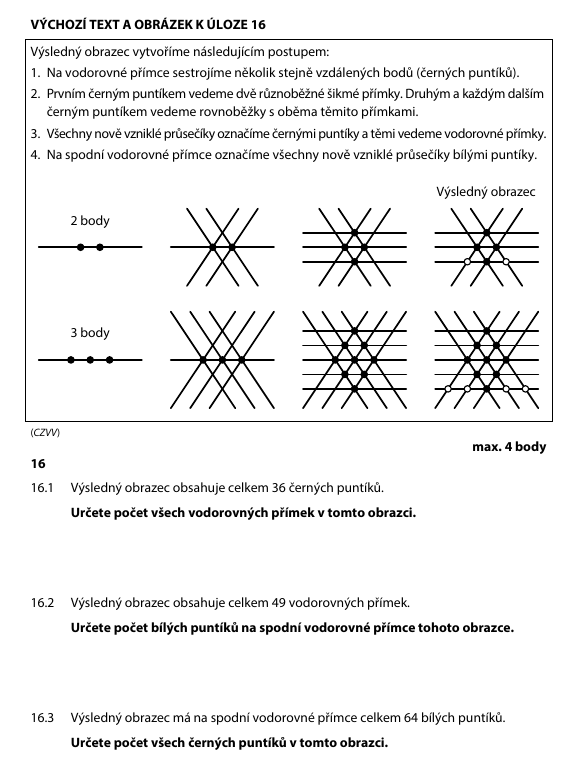
\includegraphics[width=0.6\textwidth]{opakujici_se_uloha}
\end{figure}


\section{Tvorba úloh vlastní sbírky}

Pro vlastní sbírku jsme se rozhodli tvořit úlohy pro 8leté obory. Bylo to zčásti kvůli typu úloh které obsahují, a zčásti kvůli tomu že sám studuji 8letý obor.

Úlohy jsme vytvářeli podle poznámek. Často jsou vysoce inspirované úlohami, které se v pravých zkouškách objevily.

Tvořené úlohy se liší od úloh CERMAT hlavně vzhledem, který je barevný, veselejší a přehlednější, a tím, že formát odpovědi tvořených úloh je otevřený. Student tak nemá na výběr z určitých možností a nemůže si tak tipovat.

Úlohy CERMAT mají často na výběr z odpovědí A-E, nejspíš proto že se pak dají jednodušeji opravovat.

Další rozdíl je využití geometrického zápisu, které CERMAT nevyužívá. Pro jistotu se před sbírkou vyskytuje přehled vysvětlující co která značka znamená.

Úlohy jsou tvořeny v programu GeoGebra. Z něj jsou exportovány do formátu PDF a vloženy do sbírky. Stereometrické úlohy jsou exportovány do formátu PNG, jelikož 3d GeoGebra nepodporuje ani PDF ani jiné vektorové formáty.

V obrázky úloh nemají popisky kvůli vzhledu. Obrázky bez popisků jsou tvořeny autorem.



    \singlespacing
    \chapter{Sbírka}

\subsubsection{Geometrický zápis}
\begin{tabular}{|c|p{0.7\linewidth}|}
    \hline
    $\triangle$ABC                                         & Trojúhelník ABC                                                     \\ \hline
    $\square$EFGH                                          & Čtverec EFGH                                                        \\ \hline
    $\rectangle$IJKL                                       & Obdélník IJKL                                                       \\ \hline
    $\lvert \text{MN} \rvert$                              & Vzdálenost mezi body M a N                                          \\ \hline
    $\overline{\text{OP}}$                                 & Úsečka OP                                                           \\ \hline
    $\overrightarrow{\text{QR}}$                           & Polopřímka QR                                                       \\ \hline
    $\overleftrightarrow{\text{ST}}$                       & Přímka určená body ST                                               \\ \hline
    $\overleftrightarrow{\text{u}}$                        & Přímka u                                                            \\ \hline
    $\lvert \text{V} \overleftrightarrow{\text{w}} \rvert$ & Vzdálenost mezi bodem V a přímkou W                                 \\ \hline
    $\angle \alpha $                                       & Úhel $\alpha$                                                       \\ \hline
    $ x \perp \overline{\text{YZ}} $                       & Přímka x je kolmá na úsečku YZ                                      \\ \hline
    $a \| b$                                               & Přímka a je rovnoběžná s přímkou b                                  \\ \hline
    $\lvert \text{CD} \rvert = \lvert \text{EF} \rvert$    & Vzdálenost mezi body A a B se rovná vzdálenosti mezi body C a D     \\ \hline
    $\lvert \text{GH} \rvert > \lvert \text{IJ} \rvert$    & Vzdálenost mezi body G a H je větší než vzdálenosti mezi body I a J \\ \hline
\end{tabular}

\newpage
\input{sbirka/8leté}

    \onehalfspacing
    \chapter*{Závěr}
\addcontentsline{toc}{chapter}{Závěr}

Při tvoření sbírky mi došlo

%%% Seznam použité literatury
    %%% Seznam použité literatury (bibliografie)
%%%
%%% Pro vytváření bibliografie používáme bibTeX. Ten zpracovává
%%% citace v textu (např. makro \cite{...}) a vyhledává k nim literaturu
%%% v souboru literatura.bib.
%%%
%%% Příkaz \bibliographystyle určuje, jakým stylem budou citovány odkazy
%%% v textu. V závorce je název zvoleného souboru .bst. Styly plainnat
%%% a unsrt jsou standardní součástí latexových distribucí. Styl czplainnat
%%% je dodáván s touto šablonou a bibTeX ho hledá v aktuálním adresáři.

% \bibliographystyle{czplainnat}    %% Autor (rok) s českými spojkami
% \bibliographystyle{plainnat}    %% Autor (rok) s anglickými spojkami
\bibliographystyle{unsrt}       %% [číslo]

\nocite{*}

\renewcommand{\bibname}{Zdroje}

%%% Vytvoření seznamu literatury. Pozor, pokud jste necitovali ani jednu
%%% položku, seznam se automaticky vynechá.

\bibliography{zdroje}


    \addcontentsline{toc}{chapter}{Seznam obrázků}
    \listoffigures
    \newpage
    \addcontentsline{toc}{chapter}{Seznam tabulek}
    \listoftables
    \openright
\end{document}
